\documentclass{article}\usepackage[]{graphicx}\usepackage[]{color}
% maxwidth is the original width if it is less than linewidth
% otherwise use linewidth (to make sure the graphics do not exceed the margin)
\makeatletter
\def\maxwidth{ %
  \ifdim\Gin@nat@width>\linewidth
    \linewidth
  \else
    \Gin@nat@width
  \fi
}
\makeatother

\definecolor{fgcolor}{rgb}{0.345, 0.345, 0.345}
\newcommand{\hlnum}[1]{\textcolor[rgb]{0.686,0.059,0.569}{#1}}%
\newcommand{\hlstr}[1]{\textcolor[rgb]{0.192,0.494,0.8}{#1}}%
\newcommand{\hlcom}[1]{\textcolor[rgb]{0.678,0.584,0.686}{\textit{#1}}}%
\newcommand{\hlopt}[1]{\textcolor[rgb]{0,0,0}{#1}}%
\newcommand{\hlstd}[1]{\textcolor[rgb]{0.345,0.345,0.345}{#1}}%
\newcommand{\hlkwa}[1]{\textcolor[rgb]{0.161,0.373,0.58}{\textbf{#1}}}%
\newcommand{\hlkwb}[1]{\textcolor[rgb]{0.69,0.353,0.396}{#1}}%
\newcommand{\hlkwc}[1]{\textcolor[rgb]{0.333,0.667,0.333}{#1}}%
\newcommand{\hlkwd}[1]{\textcolor[rgb]{0.737,0.353,0.396}{\textbf{#1}}}%
\let\hlipl\hlkwb

\usepackage{framed}
\makeatletter
\newenvironment{kframe}{%
 \def\at@end@of@kframe{}%
 \ifinner\ifhmode%
  \def\at@end@of@kframe{\end{minipage}}%
  \begin{minipage}{\columnwidth}%
 \fi\fi%
 \def\FrameCommand##1{\hskip\@totalleftmargin \hskip-\fboxsep
 \colorbox{shadecolor}{##1}\hskip-\fboxsep
     % There is no \\@totalrightmargin, so:
     \hskip-\linewidth \hskip-\@totalleftmargin \hskip\columnwidth}%
 \MakeFramed {\advance\hsize-\width
   \@totalleftmargin\z@ \linewidth\hsize
   \@setminipage}}%
 {\par\unskip\endMakeFramed%
 \at@end@of@kframe}
\makeatother

\definecolor{shadecolor}{rgb}{.97, .97, .97}
\definecolor{messagecolor}{rgb}{0, 0, 0}
\definecolor{warningcolor}{rgb}{1, 0, 1}
\definecolor{errorcolor}{rgb}{1, 0, 0}
\newenvironment{knitrout}{}{} % an empty environment to be redefined in TeX

\usepackage{alltt}
\usepackage{amsmath} %This allows me to use the align functionality.
                     %If you find yourself trying to replicate
                     %something you found online, ensure you're
                     %loading the necessary packages!
\usepackage{amsfonts}%Math font
\usepackage{graphicx}%For including graphics
\usepackage{hyperref}%For Hyperlinks
\hypersetup{colorlinks = true,citecolor=black}
\usepackage{natbib}        %For the bibliography
\bibliographystyle{apalike}%For the bibliography
\usepackage[margin=0.75in]{geometry}
\usepackage{float}
\IfFileExists{upquote.sty}{\usepackage{upquote}}{}
\begin{document}
\noindent \textbf{MA 354: Data Analysis I -- Fall 2021}\\%\\ gives you a new line
\noindent \textbf{Homework 4:}\vspace{1em}\\
\emph{Complete the following opportunities to use what we've talked about in class. 
These questions will be graded for correctness, communication and succinctness. 
Ensure you show your work and explain your logic in a legible and refined submission.}
%Comments -- anything after % is not put into the PDF
\begin{enumerate}
%%%%%%%%%%%%%%%%%%%%%%%%%%%%%%%%%%%%%%%%%%%%%%%%%%%%%%%%%%%%%%%%%%%%%%%%%%%%%%%
%%%%%%%%%%%%%%%%%%%%%%%%%%%%%%%%%%%%%%%%%%%%%%%%%%%%%%%%%%%%%%%%%%%%%%%%%%%%%%%
%%%%%%%%%  Question 0
%%%%%%%%%%%%%%%%%%%%%%%%%%%%%%%%%%%%%%%%%%%%%%%%%%%%%%%%%%%%%%%%%%%%%%%%%%%%%%%
%%%%%%%%%%%%%%%%%%%%%%%%%%%%%%%%%%%%%%%%%%%%%%%%%%%%%%%%%%%%%%%%%%%%%%%%%%%%%%%
\item[0.] \textbf{Complete weekly diagnostics.}
  
%%%%%%%%%%%%%%%%%%%%%%%%%%%%%%%%%%%%%%%%%%%%%%%%%%%%%%%%%%%%%%%%%%%%%%%%%%%%%%%
%%%%%%%%%%%%%%%%%%%%%%%%%%%%%%%%%%%%%%%%%%%%%%%%%%%%%%%%%%%%%%%%%%%%%%%%%%%%%%%
%%%%%%%%%  Question 1
%%%%%%%%%%%%%%%%%%%%%%%%%%%%%%%%%%%%%%%%%%%%%%%%%%%%%%%%%%%%%%%%%%%%%%%%%%%%%%%
%%%%%%%%%%%%%%%%%%%%%%%%%%%%%%%%%%%%%%%%%%%%%%%%%%%%%%%%%%%%%%%%%%%%%%%%%%%%%%%
\item On its website, Ozempic, a medication for lowering the risk of major cardiovascular 
events (e.g., heart attack, stroke, etc.), states that 
\begin{itemize}
  \item 66\% of people taking 0.5 mg Ozempic
  \item 73\% of people taking 1 mg Ozempic
  \item 40\% of people taking 100 mg Januvia
\end{itemize}
reached an A1C under 7\%, noting higher A1C is indicative of higher risk of heart disease.

\begin{enumerate}
\item Explain why this statement alone isn't enough to conclude whether there is a statistically 
significant difference among the treatments.

\begin{knitrout}
\definecolor{shadecolor}{rgb}{0.969, 0.969, 0.969}\color{fgcolor}\begin{kframe}
\begin{alltt}
\hlstr{"To assess any significant difference we need ot run a t-sample proportion test, but since we only have the information on the proportion of the people seeing beneficial affect in the above question, it is not sufficient information"}
\end{alltt}
\begin{verbatim}
## [1] "To assess any significant difference we need ot run a t-sample proportion test, but since we only have the information on the proportion of the people seeing beneficial affect in the above question, it is not sufficient information"
\end{verbatim}
\end{kframe}
\end{knitrout}
\item The statement on Ozempic's website comes from a phase 3a randomized double-blind study. 
\cite{Ahren17} reports that 409 received Ozempic (0.5 mg), 409 received Ozempic (1 mg), and 407 
received Januvia (100 mg). 
\begin{enumerate}
  \item Determine whether there is sufficient evidence of a difference in rates of attaining an 
  A1C under 7\% across treatments.
  
\begin{knitrout}
\definecolor{shadecolor}{rgb}{0.969, 0.969, 0.969}\color{fgcolor}\begin{kframe}
\begin{alltt}
\hlcom{#https://pubmed.ncbi.nlm.nih.gov/28385659/}
\hlcom{#Mean baseline HbA1c was 8·1%}
\hlcom{#2)}

\hlcom{### Remember to write about the assumptions of doing t-sample prop.test#####}
\hlcom{# Successful and total cases for 0.5 mg Ozempic}
\hlstd{x1} \hlkwb{=} \hlkwd{round}\hlstd{(}\hlnum{0.66}\hlopt{*}\hlnum{409}\hlstd{)}
\hlstd{n1} \hlkwb{=} \hlnum{409}

\hlcom{# Successful and total cases for 1 mg Ozempic}
\hlstd{x2} \hlkwb{=} \hlkwd{round}\hlstd{(}\hlnum{0.73}\hlopt{*}\hlnum{409}\hlstd{)}
\hlstd{n2} \hlkwb{=} \hlnum{409}

\hlcom{# Successful and total cases for 100 mg Januvia}
\hlstd{x3} \hlkwb{=} \hlkwd{round}\hlstd{(}\hlnum{0.4}\hlopt{*}\hlnum{407}\hlstd{)}
\hlstd{n3} \hlkwb{=} \hlnum{407}

\hlkwd{prop.test}\hlstd{(}\hlkwc{x} \hlstd{=} \hlkwd{c}\hlstd{(x1, x2, x3),} \hlkwc{n} \hlstd{=} \hlkwd{c}\hlstd{(n1, n2, n3))}
\end{alltt}
\begin{verbatim}
## 
## 	3-sample test for equality of proportions without continuity
## 	correction
## 
## data:  c(x1, x2, x3) out of c(n1, n2, n3)
## X-squared = 102.7, df = 2, p-value < 2.2e-16
## alternative hypothesis: two.sided
## sample estimates:
##    prop 1    prop 2    prop 3 
## 0.6601467 0.7310513 0.4004914
\end{verbatim}
\begin{alltt}
\hlcom{# There is a significant p-value to support a difference ()}


\hlcom{#t sample proportion test}
\hlcom{#DO IT}
\end{alltt}
\end{kframe}
\end{knitrout}
  \item Perform a follow-up analysis for comparing treatments. If you were at high risk for 
  cardiovascular events, which medication would you want to take.
\begin{knitrout}
\definecolor{shadecolor}{rgb}{0.969, 0.969, 0.969}\color{fgcolor}\begin{kframe}
\begin{alltt}
\hlkwd{pairwise.prop.test}\hlstd{(}\hlkwc{x} \hlstd{=} \hlkwd{c}\hlstd{(x1, x2, x3),} \hlkwc{n} \hlstd{=} \hlkwd{c}\hlstd{(n1, n2, n3))}
\end{alltt}
\begin{verbatim}
## 
## 	Pairwise comparisons using Pairwise comparison of proportions 
## 
## data:  c(x1, x2, x3) out of c(n1, n2, n3) 
## 
##   1       2      
## 2 0.033   -      
## 3 3.6e-13 < 2e-16
## 
## P value adjustment method: holm
\end{verbatim}
\begin{alltt}
\hlcom{# There is a significant difference between 2 and 3 and 1 and 3 success proportions. So}
\hlcom{# 1 and 2 are better than 3. But if we have alpha = 0.05 then there is also a significant }
\hlcom{# difference between 1 and 2, in which case 2 (1 mg of Ozempic) is better.}
\end{alltt}
\end{kframe}
\end{knitrout}


\end{enumerate}
\end{enumerate}
\newpage
%%%%%%%%%%%%%%%%%%%%%%%%%%%%%%%%%%%%%%%%%%%%%%%%%%%%%%%%%%%%%%%%%%%%%%%%%%%%%%%
%%%%%%%%%%%%%%%%%%%%%%%%%%%%%%%%%%%%%%%%%%%%%%%%%%%%%%%%%%%%%%%%%%%%%%%%%%%%%%%
%%%%%%%%%  Question 2
%%%%%%%%%%%%%%%%%%%%%%%%%%%%%%%%%%%%%%%%%%%%%%%%%%%%%%%%%%%%%%%%%%%%%%%%%%%%%%%
%%%%%%%%%%%%%%%%%%%%%%%%%%%%%%%%%%%%%%%%%%%%%%%%%%%%%%%%%%%%%%%%%%%%%%%%%%%%%%%
\item Is the ANOVA really robust to Normality? Equal sample size? Equal variance?
To assess this we'll check the ability of ANOVA to detect differences in a 
sample and retain the $\alpha=0.05$ across different settings. This homework 
question was motivated by \cite{Blanca17} who published a simulation study 
about ANOVA.\\

\textbf{Remark:} My professor in graduate school always told me that I didn't
have to memorize any results, I could just derive them. The data analysis
analog to this is that if we have any questions about how a model works
under a given condition (or broken assumption) we can just simulate it!
\begin{enumerate}
  \item Plot the Laplace distribution with $m=0$ and $s=2$; the PDF
  of this distribution is cataloged in \texttt{R} as \texttt{dlaplace()} 
  in the rmutil package, which you'll need to install and load. Superimpose
  the graph of the Gaussian distribution with $\mu=0$ and $\sigma=2$. Comment
  on the differences you see and what you think might happen if the data 
  are Laplace distributed instead of the Gaussian distribution.
  \item Conduct a simulation study using the Laplace distribution. To do so, 
  complete the following 1000 times and report the proportion of times the
  data lead to a rejection of the null hypothesis.\\
\begin{knitrout}
\definecolor{shadecolor}{rgb}{0.969, 0.969, 0.969}\color{fgcolor}\begin{kframe}
\begin{alltt}
\hlkwd{library}\hlstd{(rmutil)}
\end{alltt}


{\ttfamily\noindent\itshape\color{messagecolor}{\#\# \\\#\# Attaching package: 'rmutil'}}

{\ttfamily\noindent\itshape\color{messagecolor}{\#\# The following object is masked from 'package:stats':\\\#\# \\\#\# \ \ \ \ nobs}}

{\ttfamily\noindent\itshape\color{messagecolor}{\#\# The following objects are masked from 'package:base':\\\#\# \\\#\# \ \ \ \ as.data.frame, units}}\begin{alltt}
\hlkwd{library}\hlstd{(tidyverse)}
\end{alltt}


{\ttfamily\noindent\itshape\color{messagecolor}{\#\# Registered S3 method overwritten by 'httr':\\\#\# \ \ method \ \ \ \ \ \ \ \ from \ \\\#\# \ \ print.response rmutil}}

{\ttfamily\noindent\itshape\color{messagecolor}{\#\# -- Attaching packages --------------------------------------- tidyverse 1.3.1 --}}

{\ttfamily\noindent\itshape\color{messagecolor}{\#\# v ggplot2 3.3.5 \ \ \ \ v purrr \ \ 0.3.4\\\#\# v tibble \ 3.1.4 \ \ \ \ v dplyr \ \ 1.0.7\\\#\# v tidyr \ \ 1.1.3 \ \ \ \ v stringr 1.4.0\\\#\# v readr \ \ 2.0.1 \ \ \ \ v forcats 0.5.1}}

{\ttfamily\noindent\itshape\color{messagecolor}{\#\# -- Conflicts ------------------------------------------ tidyverse\_conflicts() --\\\#\# x dplyr::filter() \ masks stats::filter()\\\#\# x dplyr::lag() \ \ \ \ masks stats::lag()\\\#\# x tidyr::nesting() masks rmutil::nesting()}}\begin{alltt}
\hlstd{ggdat} \hlkwb{<-} \hlkwd{data.frame}\hlstd{(}\hlkwc{x}\hlstd{=}\hlkwd{seq}\hlstd{(}\hlopt{-}\hlnum{5}\hlstd{,} \hlnum{5}\hlstd{,} \hlkwc{length.out}\hlstd{=}\hlnum{5000}\hlstd{))}\hlopt
  \hlkwd{mutate}\hlstd{(}\hlkwc{f}\hlstd{=}\hlkwd{dlaplace}\hlstd{(x,} \hlkwc{m}\hlstd{=}\hlnum{0}\hlstd{,} \hlkwc{s}\hlstd{=}\hlnum{2}\hlstd{),}
         \hlkwc{f1}\hlstd{=}\hlkwd{dnorm}\hlstd{(x,} \hlkwc{mean}\hlstd{=}\hlnum{0}\hlstd{,} \hlkwc{sd}\hlstd{=}\hlnum{2}\hlstd{))}

\hlcom{#set the legend}
\hlkwd{ggplot}\hlstd{(ggdat,} \hlkwd{aes}\hlstd{(}\hlkwc{x}\hlstd{=x,} \hlkwc{y}\hlstd{=f))}\hlopt{+}
  \hlkwd{geom_line}\hlstd{(}\hlkwc{color}\hlstd{=}\hlstr{"blue"}\hlstd{)}\hlopt{+}
  \hlkwd{geom_line}\hlstd{(}\hlkwd{aes}\hlstd{(}\hlkwc{y}\hlstd{=f1),} \hlkwc{color}\hlstd{=}\hlstr{"red"}\hlstd{)}
\end{alltt}
\end{kframe}
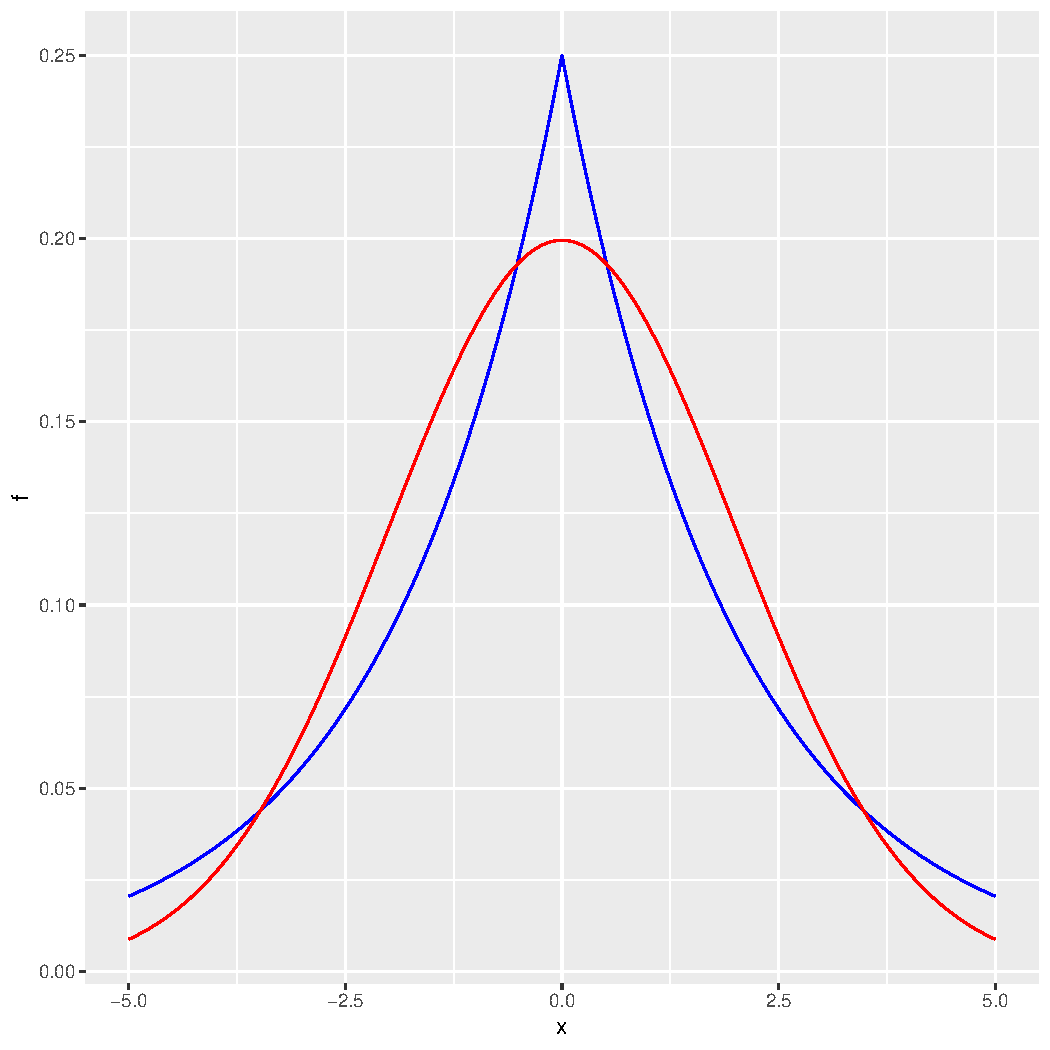
\includegraphics[width=\maxwidth]{figure/unnamed-chunk-4-1} 
\end{knitrout}
  
  The most efficient way to complete this question (including the other parts)
  is to write a function that completes the following. 
  \begin{itemize}
    \item \textbf{Input:} 
    \begin{itemize}
      \item \texttt{rand.n=FALSE} -- a logical object denoting whether the sample
                                     size is random or not. False by default.
                                     See part (f).
      \item \texttt{rand.s=FALSE} -- a logical object denoting whether the dispersion
                                     equal or not not. False by default. See part (g).
      \item \texttt{equal.m=TRUE} -- a logical object denoting whether the location
                                     parameters should be equal (part b) or different 
                                     (part c). TRUE by default. 
      \item \texttt{n=5} -- the desired sample size if not random. Five by default.
    \end{itemize}
    \item \textbf{Loop the following tasks 1000 times:}
    \begin{itemize}
      \item Generate $t=4$ samples of size $n$ drawn independently from the 
        laplace distribution with $m$ and $s$ which can be done using 
        \texttt{rlaplace()} function from the rmutil package \citep{rmutil}. Specify
        $n$, $m$, and $s$ based on the values of the
        logical variables described above.
      \item Perform the ANOVA procedure on these generated data.
      \item Store whether the test resulted in a rejected null hypothesis or not.
    \end{itemize}
    \item \textbf{Return:}
    \begin{itemize}
      \item Your function should return the proportion of the 1000 ANOVA tests
      that resulted in a rejected null hypothesis.
    \end{itemize}
  \end{itemize}
    Comment on the results of this simulation completed in the default case where
  $m_1=m_2=m_3=m_4=0$, $s_1=s_2=s_3=s_4=2$, and $n_1=n_2=n_3=n_4=5$
  
\begin{knitrout}
\definecolor{shadecolor}{rgb}{0.969, 0.969, 0.969}\color{fgcolor}\begin{kframe}
\begin{alltt}
\hlkwd{library}\hlstd{(rstatix)}
\end{alltt}


{\ttfamily\noindent\itshape\color{messagecolor}{\#\# \\\#\# Attaching package: 'rstatix'}}

{\ttfamily\noindent\itshape\color{messagecolor}{\#\# The following object is masked from 'package:stats':\\\#\# \\\#\# \ \ \ \ filter}}\begin{alltt}
\hlstd{aovFunc} \hlkwb{<-} \hlkwa{function}\hlstd{(}\hlkwc{rand.n}\hlstd{=}\hlnum{FALSE}\hlstd{,} \hlkwc{rand.s}\hlstd{=}\hlnum{FALSE}\hlstd{,} \hlkwc{equal.m}\hlstd{=}\hlnum{TRUE}\hlstd{,} \hlkwc{n}\hlstd{=}\hlnum{5}\hlstd{,} \hlkwc{loop}\hlstd{=}\hlnum{0}\hlstd{,}
                    \hlkwc{welch}\hlstd{=}\hlnum{FALSE}\hlstd{)\{}
  \hlstd{alpha}\hlkwb{<-}\hlnum{0.05}
  \hlstd{count}\hlkwb{=}\hlnum{0}
  \hlkwa{if}\hlstd{(rand.n)\{}
    \hlstd{n1}\hlkwb{=}\hlkwd{round}\hlstd{(}\hlkwd{runif}\hlstd{(}\hlnum{1}\hlstd{,} \hlkwc{min}\hlstd{=}\hlnum{5}\hlstd{,} \hlkwc{max}\hlstd{=}\hlnum{100}\hlstd{),}\hlnum{0}\hlstd{)}
    \hlstd{n2}\hlkwb{=}\hlkwd{round}\hlstd{(}\hlkwd{runif}\hlstd{(}\hlnum{1}\hlstd{,} \hlkwc{min}\hlstd{=}\hlnum{5}\hlstd{,} \hlkwc{max}\hlstd{=}\hlnum{100}\hlstd{),}\hlnum{0}\hlstd{)}
    \hlstd{n3}\hlkwb{=}\hlkwd{round}\hlstd{(}\hlkwd{runif}\hlstd{(}\hlnum{1}\hlstd{,} \hlkwc{min}\hlstd{=}\hlnum{5}\hlstd{,} \hlkwc{max}\hlstd{=}\hlnum{100}\hlstd{),}\hlnum{0}\hlstd{)}
    \hlstd{n4}\hlkwb{=}\hlkwd{round}\hlstd{(}\hlkwd{runif}\hlstd{(}\hlnum{1}\hlstd{,} \hlkwc{min}\hlstd{=}\hlnum{5}\hlstd{,} \hlkwc{max}\hlstd{=}\hlnum{100}\hlstd{),}\hlnum{0}\hlstd{)}
  \hlstd{\}}
  \hlkwa{else}\hlstd{\{}
    \hlstd{n1}\hlkwb{=}\hlstd{n}
    \hlstd{n2}\hlkwb{=}\hlstd{n}
    \hlstd{n3}\hlkwb{=}\hlstd{n}
    \hlstd{n4}\hlkwb{=}\hlstd{n}
  \hlstd{\}}

  \hlkwa{if}\hlstd{(rand.s)\{}
    \hlcom{#DOUBLE CHECK WITH PROFESSOR}
    \hlstd{s1}\hlkwb{=}\hlkwd{rgamma}\hlstd{(}\hlnum{1}\hlstd{,} \hlnum{2}\hlstd{,} \hlnum{1}\hlstd{)}
    \hlstd{s2}\hlkwb{=}\hlkwd{rgamma}\hlstd{(}\hlnum{1}\hlstd{,} \hlnum{2}\hlstd{,} \hlnum{1}\hlstd{)}
    \hlstd{s3}\hlkwb{=}\hlkwd{rgamma}\hlstd{(}\hlnum{1}\hlstd{,} \hlnum{2}\hlstd{,} \hlnum{1}\hlstd{)}
    \hlstd{s4}\hlkwb{=}\hlkwd{rgamma}\hlstd{(}\hlnum{1}\hlstd{,} \hlnum{2}\hlstd{,} \hlnum{1}\hlstd{)}
  \hlstd{\}}\hlkwa{else}\hlstd{\{}
    \hlstd{s1}\hlkwb{=}\hlnum{1}
    \hlstd{s2}\hlkwb{=}\hlnum{1}
    \hlstd{s3}\hlkwb{=}\hlnum{1}
    \hlstd{s4}\hlkwb{=}\hlnum{1}
  \hlstd{\}}
  \hlkwa{for}\hlstd{(i} \hlkwa{in} \hlnum{1}\hlopt{:}\hlstd{loop)\{}
    \hlkwa{if}\hlstd{(equal.m)\{}
      \hlstd{t1}\hlkwb{<-}\hlkwd{rlaplace}\hlstd{(}\hlkwc{n}\hlstd{=n1,} \hlkwc{m}\hlstd{=}\hlnum{0}\hlstd{,} \hlkwc{s}\hlstd{=s1)}
      \hlstd{label1}\hlkwb{<-}\hlstr{"T1"}

      \hlstd{t2}\hlkwb{<-}\hlkwd{rlaplace}\hlstd{(}\hlkwc{n}\hlstd{=n2,} \hlkwc{m}\hlstd{=}\hlnum{0}\hlstd{,} \hlkwc{s}\hlstd{=s2)}
      \hlstd{label2}\hlkwb{<-}\hlstr{"T2"}

      \hlstd{t3}\hlkwb{<-}\hlkwd{rlaplace}\hlstd{(}\hlkwc{n}\hlstd{=n3,} \hlkwc{m}\hlstd{=}\hlnum{0}\hlstd{,} \hlkwc{s}\hlstd{=s3)}
      \hlstd{label3}\hlkwb{<-}\hlstr{"T3"}

      \hlstd{t4}\hlkwb{<-}\hlkwd{rlaplace}\hlstd{(}\hlkwc{n}\hlstd{=n4,} \hlkwc{m}\hlstd{=}\hlnum{0}\hlstd{,} \hlkwc{s}\hlstd{=s4)}
      \hlstd{label4}\hlkwb{<-}\hlstr{"T4"}
    \hlstd{\}}

    \hlkwa{else}\hlstd{\{}
      \hlstd{t1}\hlkwb{<-}\hlkwd{rlaplace}\hlstd{(}\hlkwc{n}\hlstd{=n1,} \hlkwc{m}\hlstd{=}\hlnum{0}\hlstd{,} \hlkwc{s}\hlstd{=s1)}
      \hlstd{label1}\hlkwb{<-}\hlstr{"T1"}

      \hlstd{t2}\hlkwb{<-}\hlkwd{rlaplace}\hlstd{(}\hlkwc{n}\hlstd{=n2,} \hlkwc{m}\hlstd{=}\hlnum{0}\hlstd{,} \hlkwc{s}\hlstd{=s2)}
      \hlstd{label2}\hlkwb{<-}\hlstr{"T2"}

      \hlstd{t3}\hlkwb{<-}\hlkwd{rlaplace}\hlstd{(}\hlkwc{n}\hlstd{=n3,} \hlkwc{m}\hlstd{=}\hlnum{0}\hlstd{,} \hlkwc{s}\hlstd{=s3)}
      \hlstd{label3}\hlkwb{<-}\hlstr{"T3"}

      \hlstd{t4}\hlkwb{<-}\hlkwd{rlaplace}\hlstd{(}\hlkwc{n}\hlstd{=n4,} \hlkwc{m}\hlstd{=}\hlnum{1}\hlstd{,} \hlkwc{s}\hlstd{=s4)}
      \hlstd{label4}\hlkwb{<-}\hlstr{"T4"}
    \hlstd{\}}

    \hlstd{dat}\hlkwb{<-}\hlkwd{data.frame}\hlstd{(}\hlkwc{value}\hlstd{=}\hlkwd{c}\hlstd{(t1, t2, t3, t4),}
                    \hlkwc{group}\hlstd{=}\hlkwd{c}\hlstd{(}\hlkwd{rep}\hlstd{(}\hlkwd{c}\hlstd{(}\hlstr{"T1"}\hlstd{,} \hlstr{"T2"}\hlstd{,} \hlstr{"T3"}\hlstd{,} \hlstr{"T4"}\hlstd{),}
                                                         \hlkwc{times}\hlstd{=}\hlkwd{c}\hlstd{(}\hlkwd{length}\hlstd{(t1),}
                                                                 \hlkwd{length}\hlstd{(t2),}
                                                                 \hlkwd{length}\hlstd{(t3),}
                                                                 \hlkwd{length}\hlstd{(t4)))))}

    \hlkwa{if}\hlstd{(}\hlopt{!}\hlstd{welch)\{}
      \hlstd{anova}\hlkwb{<-}\hlkwd{summary}\hlstd{(}\hlkwd{aov}\hlstd{(value}\hlopt{~}\hlstd{group,} \hlkwc{data}\hlstd{=dat))}
      \hlstd{sum_test} \hlkwb{<-} \hlkwd{unlist}\hlstd{((anova))}
      \hlstd{p.value}\hlkwb{<-}\hlstd{sum_test[}\hlstr{"Pr(>F)1"}\hlstd{]}
      \hlcom{#print(p.value) #bugtest}
    \hlstd{\}}\hlkwa{else}\hlstd{\{}
      \hlstd{anova_w}\hlkwb{<-}\hlkwd{welch_anova_test}\hlstd{(value}\hlopt{~}\hlstd{group,} \hlkwc{data}\hlstd{=dat)}
      \hlstd{p.value}\hlkwb{<-}\hlstd{anova_w}\hlopt{$}\hlstd{p}
    \hlstd{\}}

    \hlkwa{if}\hlstd{(p.value}\hlopt{<}\hlnum{0.05}\hlstd{)\{}
     \hlstd{count}\hlkwb{=}\hlstd{count}\hlopt{+}\hlnum{1}
    \hlstd{\}}
  \hlstd{\}}
  \hlstd{count}\hlopt{/}\hlstd{loop}
\hlstd{\}}
\hlkwd{aovFunc}\hlstd{(}\hlkwc{loop}\hlstd{=}\hlnum{100}\hlstd{)}
\end{alltt}
\begin{verbatim}
## [1] 0.02
\end{verbatim}
\end{kframe}
\end{knitrout}

  \item Repeat the simulation study in (b-d), except with different means; i.e.,
  $m_1=m_2=m_3=0$, and $m_4=1$. Comment on the results of this simulation.

\begin{knitrout}
\definecolor{shadecolor}{rgb}{0.969, 0.969, 0.969}\color{fgcolor}\begin{kframe}
\begin{alltt}
\hlkwd{aovFunc}\hlstd{(}\hlkwc{equal.m}\hlstd{=}\hlnum{FALSE}\hlstd{,} \hlkwc{loop}\hlstd{=}\hlnum{100}\hlstd{)}
\end{alltt}
\begin{verbatim}
## [1] 0.09
\end{verbatim}
\end{kframe}
\end{knitrout}
\item Repeat the simulation study in (b-c), except with $n=15$. Comment on the results of this simulation.
\begin{knitrout}
\definecolor{shadecolor}{rgb}{0.969, 0.969, 0.969}\color{fgcolor}\begin{kframe}
\begin{alltt}
\hlkwd{aovFunc}\hlstd{(}\hlkwc{equal.m}\hlstd{=}\hlnum{TRUE}\hlstd{,} \hlkwc{loop}\hlstd{=}\hlnum{100}\hlstd{,} \hlkwc{n}\hlstd{=}\hlnum{15}\hlstd{)}
\end{alltt}
\begin{verbatim}
## [1] 0.04
\end{verbatim}
\begin{alltt}
\hlkwd{aovFunc}\hlstd{(}\hlkwc{equal.m}\hlstd{=}\hlnum{FALSE}\hlstd{,} \hlkwc{loop}\hlstd{=}\hlnum{100}\hlstd{,} \hlkwc{n}\hlstd{=}\hlnum{15}\hlstd{)}
\end{alltt}
\begin{verbatim}
## [1] 0.5
\end{verbatim}
\end{kframe}
\end{knitrout}
  \item Repeat the simulation study in (b-c), except with $n=50$.
  Comment on the results of this simulation.
\begin{knitrout}
\definecolor{shadecolor}{rgb}{0.969, 0.969, 0.969}\color{fgcolor}\begin{kframe}
\begin{alltt}
\hlkwd{aovFunc}\hlstd{(}\hlkwc{equal.m}\hlstd{=}\hlnum{TRUE}\hlstd{,} \hlkwc{loop}\hlstd{=}\hlnum{100}\hlstd{,} \hlkwc{n}\hlstd{=}\hlnum{50}\hlstd{)}
\end{alltt}
\begin{verbatim}
## [1] 0.05
\end{verbatim}
\begin{alltt}
\hlkwd{aovFunc}\hlstd{(}\hlkwc{equal.m}\hlstd{=}\hlnum{FALSE}\hlstd{,} \hlkwc{loop}\hlstd{=}\hlnum{100}\hlstd{,} \hlkwc{n}\hlstd{=}\hlnum{50}\hlstd{)}
\end{alltt}
\begin{verbatim}
## [1] 1
\end{verbatim}
\end{kframe}
\end{knitrout}
\item Repeat (b-e), except randomly select the sample size for each 
group by selecting $n$ from the uniform(5,100) distribution. This 
will help us assess the robustness of the equal sample size assumption
in the Laplace population distribution case. Comment on the results of 
this simulation.
\begin{knitrout}
\definecolor{shadecolor}{rgb}{0.969, 0.969, 0.969}\color{fgcolor}\begin{kframe}
\begin{alltt}
\hlkwd{aovFunc}\hlstd{(}\hlkwc{equal.m}\hlstd{=}\hlnum{TRUE}\hlstd{,} \hlkwc{rand.n}\hlstd{=}\hlnum{TRUE}\hlstd{,} \hlkwc{loop}\hlstd{=}\hlnum{100}\hlstd{)}
\end{alltt}
\begin{verbatim}
## [1] 0.05
\end{verbatim}
\begin{alltt}
\hlkwd{aovFunc}\hlstd{(}\hlkwc{equal.m}\hlstd{=}\hlnum{FALSE}\hlstd{,} \hlkwc{rand.n}\hlstd{=}\hlnum{TRUE}\hlstd{,} \hlkwc{loop}\hlstd{=}\hlnum{100}\hlstd{)}
\end{alltt}
\begin{verbatim}
## [1] 0.95
\end{verbatim}
\end{kframe}
\end{knitrout}
\item Repeat (b-f), except randomly select the dispersion for each 
  group by selecting $s$ from the gamma(2,1) distribution. This 
  will help us assess the robustness of the equal variance assumption
  in the Laplace population distribution case. Comment on the results of 
  this simulation.
\begin{knitrout}
\definecolor{shadecolor}{rgb}{0.969, 0.969, 0.969}\color{fgcolor}\begin{kframe}
\begin{alltt}
\hlkwd{aovFunc}\hlstd{(}\hlkwc{equal.m}\hlstd{=}\hlnum{TRUE}\hlstd{,} \hlkwc{rand.n}\hlstd{=}\hlnum{TRUE}\hlstd{,} \hlkwc{rand.s}\hlstd{=}\hlnum{TRUE}\hlstd{,} \hlkwc{loop}\hlstd{=}\hlnum{100}\hlstd{)}
\end{alltt}
\begin{verbatim}
## [1] 0.1
\end{verbatim}
\begin{alltt}
\hlkwd{aovFunc}\hlstd{(}\hlkwc{equal.m}\hlstd{=}\hlnum{FALSE}\hlstd{,} \hlkwc{rand.n}\hlstd{=}\hlnum{TRUE}\hlstd{,} \hlkwc{rand.s}\hlstd{=}\hlnum{TRUE}\hlstd{,} \hlkwc{loop}\hlstd{=}\hlnum{100}\hlstd{)}
\end{alltt}
\begin{verbatim}
## [1] 0.1
\end{verbatim}
\end{kframe}
\end{knitrout}
\item Write a loop that conducts this simulation when (1) $s$ is fixed and (2) 
when $s$ is random, for the case where the means are unequal. The loop should be 
with respect to $n$, and should run for $n=5$ to $n=200$.\\

\begin{knitrout}
\definecolor{shadecolor}{rgb}{0.969, 0.969, 0.969}\color{fgcolor}\begin{kframe}
\begin{alltt}
\hlcom{# results<-c()}
\hlcom{# n<-10:50}
\hlcom{# y1<-c()}
\hlcom{# y2<-c()}
\hlcom{# y3<-c()}
\hlcom{# }
\hlcom{# for(i in 10:50)\{}
\hlcom{#   print(i)}
\hlcom{#   unequal<-aovFunc(equal.m=FALSE, rand.s=TRUE, loop=100, n=i)}
\hlcom{#   y1<-c(y1, unequal)}
\hlcom{#   equal<-aovFunc(equal.m=FALSE, rand.s=FALSE, loop=100, n=i)}
\hlcom{#   y2<-c(y2, equal)}
\hlcom{#   }
\hlcom{#   wUnequal<-aovFunc(equal.m=FALSE, rand.s=TRUE, loop=100, n=i, welch=T)}
\hlcom{#   y3<-c(y3, wUnequal)}
\hlcom{# \}}
\hlcom{# }
\hlcom{# ggdat<-data.frame(x=n, equal.s=y2, unequal.s=y1,}
\hlcom{#                   welch=y3)}
\hlcom{# ggplot(ggdat, aes(x=x))+}
\hlcom{#   geom_line(aes(y=equal.s), color="red")+}
\hlcom{#   geom_line(aes(y=unequal.s), color="blue")+}
\hlcom{#   geom_line(aes(y=welch), color="black")+}
\hlcom{#   labs(title="Everybody hates Welch")}
\end{alltt}
\end{kframe}
\end{knitrout}
\textbf{Note:} This can take some computation time, you'll want to run it and save 
the image as a .pdf so you can load it instead of rerunning the code.
\end{enumerate}
\newpage
%%%%%%%%%%%%%%%%%%%%%%%%%%%%%%%%%%%%%%%%%%%%%%%%%%%%%%%%%%%%%%%%%%%%%%%%%%%%%%%
%%%%%%%%%%%%%%%%%%%%%%%%%%%%%%%%%%%%%%%%%%%%%%%%%%%%%%%%%%%%%%%%%%%%%%%%%%%%%%%
%%%%%%%%%  Question 3
%%%%%%%%%%%%%%%%%%%%%%%%%%%%%%%%%%%%%%%%%%%%%%%%%%%%%%%%%%%%%%%%%%%%%%%%%%%%%%%
%%%%%%%%%%%%%%%%%%%%%%%%%%%%%%%%%%%%%%%%%%%%%%%%%%%%%%%%%%%%%%%%%%%%%%%%%%%%%%%
  \item Complete the following parts. This will lead you through the simulation
  of data, fitting regression lines and evaluating the assumptions.
  \begin{enumerate}
  \item Fit a model to the following simulated data. Make observations about
  the model equation and the Pearson correlation.
\begin{knitrout}
\definecolor{shadecolor}{rgb}{0.969, 0.969, 0.969}\color{fgcolor}\begin{kframe}
\begin{alltt}
\hlstd{n}\hlkwb{=}\hlnum{500}
\hlstd{x}\hlkwb{<-}\hlkwd{sample}\hlstd{(}\hlkwc{x} \hlstd{=} \hlkwd{seq}\hlstd{(}\hlnum{0}\hlstd{,}\hlnum{5}\hlstd{,}\hlnum{0.01}\hlstd{),} \hlkwc{size}\hlstd{=n,} \hlkwc{replace}\hlstd{=T)}
\hlstd{y}\hlkwb{<-}\hlnum{5}\hlopt{*}\hlstd{x} \hlopt{+} \hlnum{3}

\hlstd{ggdat}\hlkwb{<-}\hlkwd{data.frame}\hlstd{(}\hlkwc{x}\hlstd{=x,} \hlkwc{y}\hlstd{=y)}
\hlkwd{ggplot}\hlstd{(ggdat,} \hlkwd{aes}\hlstd{(}\hlkwc{x}\hlstd{=x,} \hlkwc{y}\hlstd{=y))}\hlopt{+}
  \hlkwd{geom_smooth}\hlstd{(}\hlkwc{color}\hlstd{=}\hlstr{"blue"}\hlstd{,}
              \hlkwc{method}\hlstd{=}\hlstr{"lm"}\hlstd{,}
              \hlkwc{formula}\hlstd{=y}\hlopt{~}\hlstd{x)}\hlopt{+}
  \hlkwd{geom_point}\hlstd{(}\hlkwc{shape}\hlstd{=}\hlnum{1}\hlstd{,}
             \hlkwc{alpha}\hlstd{=}\hlnum{.3}\hlstd{)}
\end{alltt}
\end{kframe}
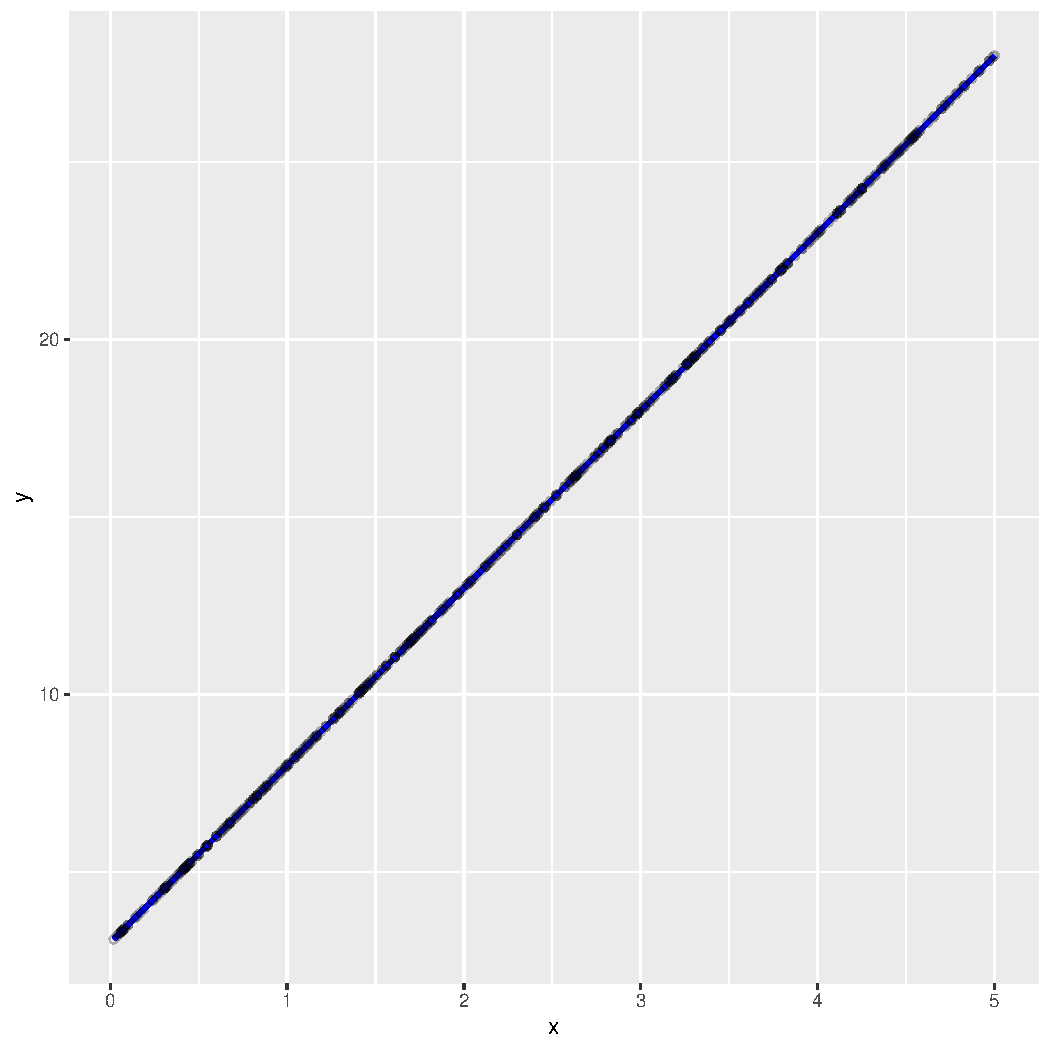
\includegraphics[width=\maxwidth]{figure/unnamed-chunk-12-1} 
\begin{kframe}\begin{alltt}
  \hlkwd{theme_bw}\hlstd{()}
\end{alltt}
\begin{verbatim}
## List of 93
##  $ line                      :List of 6
##   ..$ colour       : chr "black"
##   ..$ size         : num 0.5
##   ..$ linetype     : num 1
##   ..$ lineend      : chr "butt"
##   ..$ arrow        : logi FALSE
##   ..$ inherit.blank: logi TRUE
##   ..- attr(*, "class")= chr [1:2] "element_line" "element"
##  $ rect                      :List of 5
##   ..$ fill         : chr "white"
##   ..$ colour       : chr "black"
##   ..$ size         : num 0.5
##   ..$ linetype     : num 1
##   ..$ inherit.blank: logi TRUE
##   ..- attr(*, "class")= chr [1:2] "element_rect" "element"
##  $ text                      :List of 11
##   ..$ family       : chr ""
##   ..$ face         : chr "plain"
##   ..$ colour       : chr "black"
##   ..$ size         : num 11
##   ..$ hjust        : num 0.5
##   ..$ vjust        : num 0.5
##   ..$ angle        : num 0
##   ..$ lineheight   : num 0.9
##   ..$ margin       : 'margin' num [1:4] 0points 0points 0points 0points
##   .. ..- attr(*, "unit")= int 8
##   ..$ debug        : logi FALSE
##   ..$ inherit.blank: logi TRUE
##   ..- attr(*, "class")= chr [1:2] "element_text" "element"
##  $ title                     : NULL
##  $ aspect.ratio              : NULL
##  $ axis.title                : NULL
##  $ axis.title.x              :List of 11
##   ..$ family       : NULL
##   ..$ face         : NULL
##   ..$ colour       : NULL
##   ..$ size         : NULL
##   ..$ hjust        : NULL
##   ..$ vjust        : num 1
##   ..$ angle        : NULL
##   ..$ lineheight   : NULL
##   ..$ margin       : 'margin' num [1:4] 2.75points 0points 0points 0points
##   .. ..- attr(*, "unit")= int 8
##   ..$ debug        : NULL
##   ..$ inherit.blank: logi TRUE
##   ..- attr(*, "class")= chr [1:2] "element_text" "element"
##  $ axis.title.x.top          :List of 11
##   ..$ family       : NULL
##   ..$ face         : NULL
##   ..$ colour       : NULL
##   ..$ size         : NULL
##   ..$ hjust        : NULL
##   ..$ vjust        : num 0
##   ..$ angle        : NULL
##   ..$ lineheight   : NULL
##   ..$ margin       : 'margin' num [1:4] 0points 0points 2.75points 0points
##   .. ..- attr(*, "unit")= int 8
##   ..$ debug        : NULL
##   ..$ inherit.blank: logi TRUE
##   ..- attr(*, "class")= chr [1:2] "element_text" "element"
##  $ axis.title.x.bottom       : NULL
##  $ axis.title.y              :List of 11
##   ..$ family       : NULL
##   ..$ face         : NULL
##   ..$ colour       : NULL
##   ..$ size         : NULL
##   ..$ hjust        : NULL
##   ..$ vjust        : num 1
##   ..$ angle        : num 90
##   ..$ lineheight   : NULL
##   ..$ margin       : 'margin' num [1:4] 0points 2.75points 0points 0points
##   .. ..- attr(*, "unit")= int 8
##   ..$ debug        : NULL
##   ..$ inherit.blank: logi TRUE
##   ..- attr(*, "class")= chr [1:2] "element_text" "element"
##  $ axis.title.y.left         : NULL
##  $ axis.title.y.right        :List of 11
##   ..$ family       : NULL
##   ..$ face         : NULL
##   ..$ colour       : NULL
##   ..$ size         : NULL
##   ..$ hjust        : NULL
##   ..$ vjust        : num 0
##   ..$ angle        : num -90
##   ..$ lineheight   : NULL
##   ..$ margin       : 'margin' num [1:4] 0points 0points 0points 2.75points
##   .. ..- attr(*, "unit")= int 8
##   ..$ debug        : NULL
##   ..$ inherit.blank: logi TRUE
##   ..- attr(*, "class")= chr [1:2] "element_text" "element"
##  $ axis.text                 :List of 11
##   ..$ family       : NULL
##   ..$ face         : NULL
##   ..$ colour       : chr "grey30"
##   ..$ size         : 'rel' num 0.8
##   ..$ hjust        : NULL
##   ..$ vjust        : NULL
##   ..$ angle        : NULL
##   ..$ lineheight   : NULL
##   ..$ margin       : NULL
##   ..$ debug        : NULL
##   ..$ inherit.blank: logi TRUE
##   ..- attr(*, "class")= chr [1:2] "element_text" "element"
##  $ axis.text.x               :List of 11
##   ..$ family       : NULL
##   ..$ face         : NULL
##   ..$ colour       : NULL
##   ..$ size         : NULL
##   ..$ hjust        : NULL
##   ..$ vjust        : num 1
##   ..$ angle        : NULL
##   ..$ lineheight   : NULL
##   ..$ margin       : 'margin' num [1:4] 2.2points 0points 0points 0points
##   .. ..- attr(*, "unit")= int 8
##   ..$ debug        : NULL
##   ..$ inherit.blank: logi TRUE
##   ..- attr(*, "class")= chr [1:2] "element_text" "element"
##  $ axis.text.x.top           :List of 11
##   ..$ family       : NULL
##   ..$ face         : NULL
##   ..$ colour       : NULL
##   ..$ size         : NULL
##   ..$ hjust        : NULL
##   ..$ vjust        : num 0
##   ..$ angle        : NULL
##   ..$ lineheight   : NULL
##   ..$ margin       : 'margin' num [1:4] 0points 0points 2.2points 0points
##   .. ..- attr(*, "unit")= int 8
##   ..$ debug        : NULL
##   ..$ inherit.blank: logi TRUE
##   ..- attr(*, "class")= chr [1:2] "element_text" "element"
##  $ axis.text.x.bottom        : NULL
##  $ axis.text.y               :List of 11
##   ..$ family       : NULL
##   ..$ face         : NULL
##   ..$ colour       : NULL
##   ..$ size         : NULL
##   ..$ hjust        : num 1
##   ..$ vjust        : NULL
##   ..$ angle        : NULL
##   ..$ lineheight   : NULL
##   ..$ margin       : 'margin' num [1:4] 0points 2.2points 0points 0points
##   .. ..- attr(*, "unit")= int 8
##   ..$ debug        : NULL
##   ..$ inherit.blank: logi TRUE
##   ..- attr(*, "class")= chr [1:2] "element_text" "element"
##  $ axis.text.y.left          : NULL
##  $ axis.text.y.right         :List of 11
##   ..$ family       : NULL
##   ..$ face         : NULL
##   ..$ colour       : NULL
##   ..$ size         : NULL
##   ..$ hjust        : num 0
##   ..$ vjust        : NULL
##   ..$ angle        : NULL
##   ..$ lineheight   : NULL
##   ..$ margin       : 'margin' num [1:4] 0points 0points 0points 2.2points
##   .. ..- attr(*, "unit")= int 8
##   ..$ debug        : NULL
##   ..$ inherit.blank: logi TRUE
##   ..- attr(*, "class")= chr [1:2] "element_text" "element"
##  $ axis.ticks                :List of 6
##   ..$ colour       : chr "grey20"
##   ..$ size         : NULL
##   ..$ linetype     : NULL
##   ..$ lineend      : NULL
##   ..$ arrow        : logi FALSE
##   ..$ inherit.blank: logi TRUE
##   ..- attr(*, "class")= chr [1:2] "element_line" "element"
##  $ axis.ticks.x              : NULL
##  $ axis.ticks.x.top          : NULL
##  $ axis.ticks.x.bottom       : NULL
##  $ axis.ticks.y              : NULL
##  $ axis.ticks.y.left         : NULL
##  $ axis.ticks.y.right        : NULL
##  $ axis.ticks.length         : 'simpleUnit' num 2.75points
##   ..- attr(*, "unit")= int 8
##  $ axis.ticks.length.x       : NULL
##  $ axis.ticks.length.x.top   : NULL
##  $ axis.ticks.length.x.bottom: NULL
##  $ axis.ticks.length.y       : NULL
##  $ axis.ticks.length.y.left  : NULL
##  $ axis.ticks.length.y.right : NULL
##  $ axis.line                 : list()
##   ..- attr(*, "class")= chr [1:2] "element_blank" "element"
##  $ axis.line.x               : NULL
##  $ axis.line.x.top           : NULL
##  $ axis.line.x.bottom        : NULL
##  $ axis.line.y               : NULL
##  $ axis.line.y.left          : NULL
##  $ axis.line.y.right         : NULL
##  $ legend.background         :List of 5
##   ..$ fill         : NULL
##   ..$ colour       : logi NA
##   ..$ size         : NULL
##   ..$ linetype     : NULL
##   ..$ inherit.blank: logi TRUE
##   ..- attr(*, "class")= chr [1:2] "element_rect" "element"
##  $ legend.margin             : 'margin' num [1:4] 5.5points 5.5points 5.5points 5.5points
##   ..- attr(*, "unit")= int 8
##  $ legend.spacing            : 'simpleUnit' num 11points
##   ..- attr(*, "unit")= int 8
##  $ legend.spacing.x          : NULL
##  $ legend.spacing.y          : NULL
##  $ legend.key                :List of 5
##   ..$ fill         : chr "white"
##   ..$ colour       : logi NA
##   ..$ size         : NULL
##   ..$ linetype     : NULL
##   ..$ inherit.blank: logi TRUE
##   ..- attr(*, "class")= chr [1:2] "element_rect" "element"
##  $ legend.key.size           : 'simpleUnit' num 1.2lines
##   ..- attr(*, "unit")= int 3
##  $ legend.key.height         : NULL
##  $ legend.key.width          : NULL
##  $ legend.text               :List of 11
##   ..$ family       : NULL
##   ..$ face         : NULL
##   ..$ colour       : NULL
##   ..$ size         : 'rel' num 0.8
##   ..$ hjust        : NULL
##   ..$ vjust        : NULL
##   ..$ angle        : NULL
##   ..$ lineheight   : NULL
##   ..$ margin       : NULL
##   ..$ debug        : NULL
##   ..$ inherit.blank: logi TRUE
##   ..- attr(*, "class")= chr [1:2] "element_text" "element"
##  $ legend.text.align         : NULL
##  $ legend.title              :List of 11
##   ..$ family       : NULL
##   ..$ face         : NULL
##   ..$ colour       : NULL
##   ..$ size         : NULL
##   ..$ hjust        : num 0
##   ..$ vjust        : NULL
##   ..$ angle        : NULL
##   ..$ lineheight   : NULL
##   ..$ margin       : NULL
##   ..$ debug        : NULL
##   ..$ inherit.blank: logi TRUE
##   ..- attr(*, "class")= chr [1:2] "element_text" "element"
##  $ legend.title.align        : NULL
##  $ legend.position           : chr "right"
##  $ legend.direction          : NULL
##  $ legend.justification      : chr "center"
##  $ legend.box                : NULL
##  $ legend.box.just           : NULL
##  $ legend.box.margin         : 'margin' num [1:4] 0cm 0cm 0cm 0cm
##   ..- attr(*, "unit")= int 1
##  $ legend.box.background     : list()
##   ..- attr(*, "class")= chr [1:2] "element_blank" "element"
##  $ legend.box.spacing        : 'simpleUnit' num 11points
##   ..- attr(*, "unit")= int 8
##  $ panel.background          :List of 5
##   ..$ fill         : chr "white"
##   ..$ colour       : logi NA
##   ..$ size         : NULL
##   ..$ linetype     : NULL
##   ..$ inherit.blank: logi TRUE
##   ..- attr(*, "class")= chr [1:2] "element_rect" "element"
##  $ panel.border              :List of 5
##   ..$ fill         : logi NA
##   ..$ colour       : chr "grey20"
##   ..$ size         : NULL
##   ..$ linetype     : NULL
##   ..$ inherit.blank: logi TRUE
##   ..- attr(*, "class")= chr [1:2] "element_rect" "element"
##  $ panel.spacing             : 'simpleUnit' num 5.5points
##   ..- attr(*, "unit")= int 8
##  $ panel.spacing.x           : NULL
##  $ panel.spacing.y           : NULL
##  $ panel.grid                :List of 6
##   ..$ colour       : chr "grey92"
##   ..$ size         : NULL
##   ..$ linetype     : NULL
##   ..$ lineend      : NULL
##   ..$ arrow        : logi FALSE
##   ..$ inherit.blank: logi TRUE
##   ..- attr(*, "class")= chr [1:2] "element_line" "element"
##  $ panel.grid.major          : NULL
##  $ panel.grid.minor          :List of 6
##   ..$ colour       : NULL
##   ..$ size         : 'rel' num 0.5
##   ..$ linetype     : NULL
##   ..$ lineend      : NULL
##   ..$ arrow        : logi FALSE
##   ..$ inherit.blank: logi TRUE
##   ..- attr(*, "class")= chr [1:2] "element_line" "element"
##  $ panel.grid.major.x        : NULL
##  $ panel.grid.major.y        : NULL
##  $ panel.grid.minor.x        : NULL
##  $ panel.grid.minor.y        : NULL
##  $ panel.ontop               : logi FALSE
##  $ plot.background           :List of 5
##   ..$ fill         : NULL
##   ..$ colour       : chr "white"
##   ..$ size         : NULL
##   ..$ linetype     : NULL
##   ..$ inherit.blank: logi TRUE
##   ..- attr(*, "class")= chr [1:2] "element_rect" "element"
##  $ plot.title                :List of 11
##   ..$ family       : NULL
##   ..$ face         : NULL
##   ..$ colour       : NULL
##   ..$ size         : 'rel' num 1.2
##   ..$ hjust        : num 0
##   ..$ vjust        : num 1
##   ..$ angle        : NULL
##   ..$ lineheight   : NULL
##   ..$ margin       : 'margin' num [1:4] 0points 0points 5.5points 0points
##   .. ..- attr(*, "unit")= int 8
##   ..$ debug        : NULL
##   ..$ inherit.blank: logi TRUE
##   ..- attr(*, "class")= chr [1:2] "element_text" "element"
##  $ plot.title.position       : chr "panel"
##  $ plot.subtitle             :List of 11
##   ..$ family       : NULL
##   ..$ face         : NULL
##   ..$ colour       : NULL
##   ..$ size         : NULL
##   ..$ hjust        : num 0
##   ..$ vjust        : num 1
##   ..$ angle        : NULL
##   ..$ lineheight   : NULL
##   ..$ margin       : 'margin' num [1:4] 0points 0points 5.5points 0points
##   .. ..- attr(*, "unit")= int 8
##   ..$ debug        : NULL
##   ..$ inherit.blank: logi TRUE
##   ..- attr(*, "class")= chr [1:2] "element_text" "element"
##  $ plot.caption              :List of 11
##   ..$ family       : NULL
##   ..$ face         : NULL
##   ..$ colour       : NULL
##   ..$ size         : 'rel' num 0.8
##   ..$ hjust        : num 1
##   ..$ vjust        : num 1
##   ..$ angle        : NULL
##   ..$ lineheight   : NULL
##   ..$ margin       : 'margin' num [1:4] 5.5points 0points 0points 0points
##   .. ..- attr(*, "unit")= int 8
##   ..$ debug        : NULL
##   ..$ inherit.blank: logi TRUE
##   ..- attr(*, "class")= chr [1:2] "element_text" "element"
##  $ plot.caption.position     : chr "panel"
##  $ plot.tag                  :List of 11
##   ..$ family       : NULL
##   ..$ face         : NULL
##   ..$ colour       : NULL
##   ..$ size         : 'rel' num 1.2
##   ..$ hjust        : num 0.5
##   ..$ vjust        : num 0.5
##   ..$ angle        : NULL
##   ..$ lineheight   : NULL
##   ..$ margin       : NULL
##   ..$ debug        : NULL
##   ..$ inherit.blank: logi TRUE
##   ..- attr(*, "class")= chr [1:2] "element_text" "element"
##  $ plot.tag.position         : chr "topleft"
##  $ plot.margin               : 'margin' num [1:4] 5.5points 5.5points 5.5points 5.5points
##   ..- attr(*, "unit")= int 8
##  $ strip.background          :List of 5
##   ..$ fill         : chr "grey85"
##   ..$ colour       : chr "grey20"
##   ..$ size         : NULL
##   ..$ linetype     : NULL
##   ..$ inherit.blank: logi TRUE
##   ..- attr(*, "class")= chr [1:2] "element_rect" "element"
##  $ strip.background.x        : NULL
##  $ strip.background.y        : NULL
##  $ strip.placement           : chr "inside"
##  $ strip.text                :List of 11
##   ..$ family       : NULL
##   ..$ face         : NULL
##   ..$ colour       : chr "grey10"
##   ..$ size         : 'rel' num 0.8
##   ..$ hjust        : NULL
##   ..$ vjust        : NULL
##   ..$ angle        : NULL
##   ..$ lineheight   : NULL
##   ..$ margin       : 'margin' num [1:4] 4.4points 4.4points 4.4points 4.4points
##   .. ..- attr(*, "unit")= int 8
##   ..$ debug        : NULL
##   ..$ inherit.blank: logi TRUE
##   ..- attr(*, "class")= chr [1:2] "element_text" "element"
##  $ strip.text.x              : NULL
##  $ strip.text.y              :List of 11
##   ..$ family       : NULL
##   ..$ face         : NULL
##   ..$ colour       : NULL
##   ..$ size         : NULL
##   ..$ hjust        : NULL
##   ..$ vjust        : NULL
##   ..$ angle        : num -90
##   ..$ lineheight   : NULL
##   ..$ margin       : NULL
##   ..$ debug        : NULL
##   ..$ inherit.blank: logi TRUE
##   ..- attr(*, "class")= chr [1:2] "element_text" "element"
##  $ strip.switch.pad.grid     : 'simpleUnit' num 2.75points
##   ..- attr(*, "unit")= int 8
##  $ strip.switch.pad.wrap     : 'simpleUnit' num 2.75points
##   ..- attr(*, "unit")= int 8
##  $ strip.text.y.left         :List of 11
##   ..$ family       : NULL
##   ..$ face         : NULL
##   ..$ colour       : NULL
##   ..$ size         : NULL
##   ..$ hjust        : NULL
##   ..$ vjust        : NULL
##   ..$ angle        : num 90
##   ..$ lineheight   : NULL
##   ..$ margin       : NULL
##   ..$ debug        : NULL
##   ..$ inherit.blank: logi TRUE
##   ..- attr(*, "class")= chr [1:2] "element_text" "element"
##  - attr(*, "class")= chr [1:2] "theme" "gg"
##  - attr(*, "complete")= logi TRUE
##  - attr(*, "validate")= logi TRUE
\end{verbatim}
\begin{alltt}
  \hlcom{#put pearson on the plot}
\end{alltt}
\end{kframe}
\end{knitrout}
  \item Fit a model to the following simulated data, now with added Normal error. Make
  observations about the model equation and the Pearson correlation in relation to (a).
\begin{knitrout}
\definecolor{shadecolor}{rgb}{0.969, 0.969, 0.969}\color{fgcolor}\begin{kframe}
\begin{alltt}
\hlstd{e}\hlkwb{<-}\hlkwd{rnorm}\hlstd{(}\hlkwc{n}\hlstd{=n,}\hlkwc{mean}\hlstd{=}\hlnum{0}\hlstd{,}\hlkwc{sd}\hlstd{=}\hlnum{3}\hlstd{)}
\hlstd{y2}\hlkwb{<-}\hlnum{5}\hlopt{*}\hlstd{x} \hlopt{+} \hlnum{3} \hlopt{+} \hlstd{e}

\hlstd{ggdat}\hlkwb{<-}\hlkwd{data.frame}\hlstd{(}\hlkwc{x}\hlstd{=x,} \hlkwc{y}\hlstd{=y2)}
\hlkwd{ggplot}\hlstd{(ggdat,} \hlkwd{aes}\hlstd{(}\hlkwc{x}\hlstd{=x,} \hlkwc{y}\hlstd{=y))}\hlopt{+}
  \hlkwd{geom_smooth}\hlstd{(}\hlkwc{color}\hlstd{=}\hlstr{"blue"}\hlstd{,}
              \hlkwc{method}\hlstd{=}\hlstr{"lm"}\hlstd{,}
              \hlkwc{formula}\hlstd{=y}\hlopt{~}\hlstd{x)}\hlopt{+}
  \hlkwd{geom_point}\hlstd{(}\hlkwc{shape}\hlstd{=}\hlnum{1}\hlstd{,}
             \hlkwc{alpha}\hlstd{=}\hlnum{.3}\hlstd{)}\hlopt{+}
  \hlkwd{theme_bw}\hlstd{()}
\end{alltt}
\end{kframe}
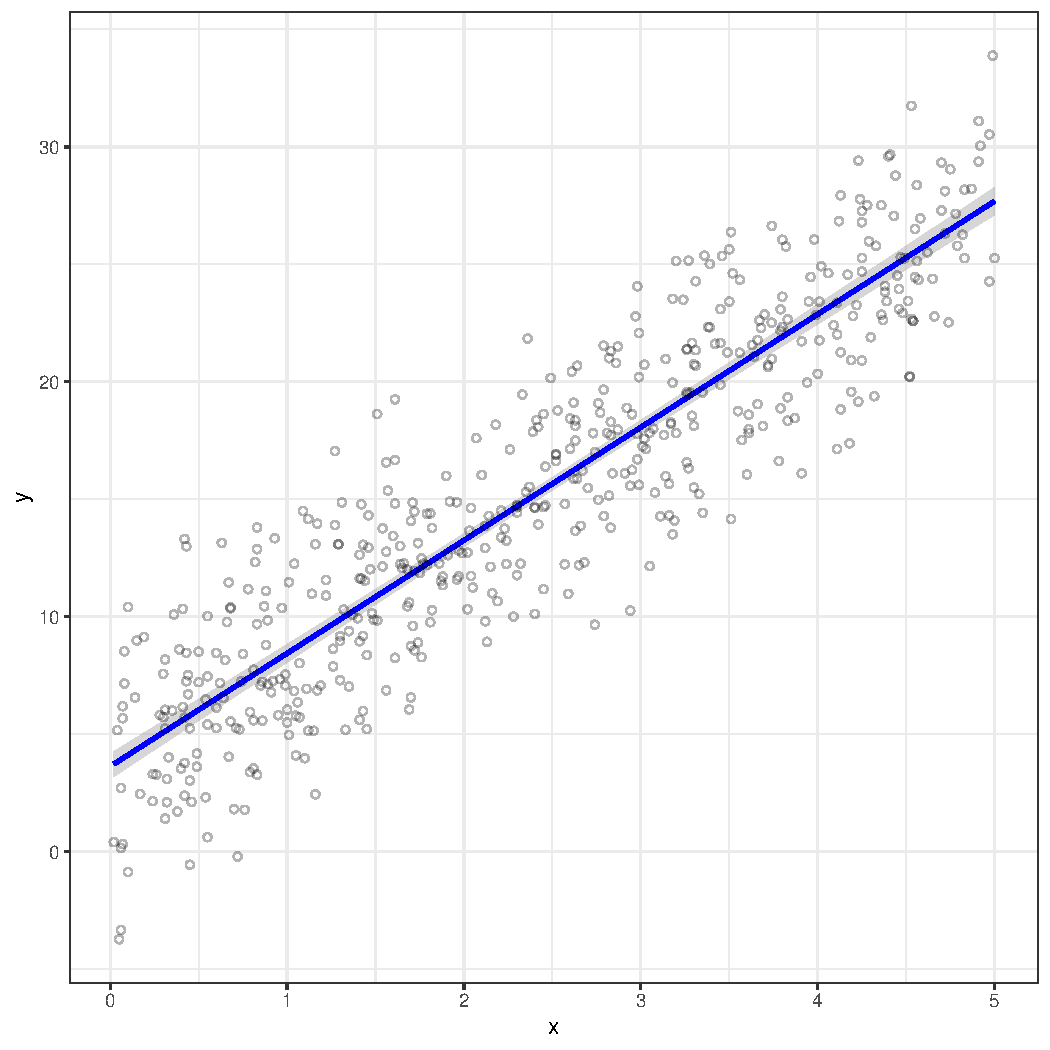
\includegraphics[width=\maxwidth]{figure/unnamed-chunk-13-1} 
\begin{kframe}\begin{alltt}
  \hlcom{#put pearson on the plot}
\hlkwd{cor}\hlstd{(x, y2,} \hlkwc{method}\hlstd{=}\hlstr{"pearson"}\hlstd{)}
\end{alltt}
\begin{verbatim}
## [1] 0.9086291
\end{verbatim}
\end{kframe}
\end{knitrout}
  \item In the model of part (b), evaluate the normality and homogeneity of error terms. Note 
  that we know both of these items to be true since we've taken $\epsilon \sim 
  \textrm{N}(\mu=0,\sigma=3)$.
\begin{knitrout}
\definecolor{shadecolor}{rgb}{0.969, 0.969, 0.969}\color{fgcolor}\begin{kframe}
\begin{alltt}
\hlcom{#not stealing your function, prof. c:}
\hlstd{plotResiduals}\hlkwb{<-}\hlkwa{function}\hlstd{(}\hlkwc{mod}\hlstd{)\{}
  \hlstd{ggdat} \hlkwb{<-} \hlkwd{data.frame}\hlstd{(}\hlkwc{y.hat} \hlstd{=} \hlkwd{fitted}\hlstd{(mod),}
                      \hlkwc{e} \hlstd{=} \hlkwd{residuals}\hlstd{(mod))}

  \hlcom{########################################}
  \hlcom{####  Fitted versus residuals}
  \hlcom{########################################}
  \hlstd{p1}\hlkwb{<-}\hlkwd{ggplot}\hlstd{(}\hlkwc{data}\hlstd{=ggdat,}\hlkwd{aes}\hlstd{(}\hlkwc{x}\hlstd{=y.hat,}\hlkwc{y}\hlstd{=e))}\hlopt{+}
    \hlkwd{geom_point}\hlstd{(}\hlkwc{shape}\hlstd{=}\hlnum{1}\hlstd{)}\hlopt{+}
    \hlkwd{geom_hline}\hlstd{(}\hlkwc{yintercept}\hlstd{=}\hlnum{0}\hlstd{,}\hlkwc{linetype}\hlstd{=}\hlstr{"dashed"}\hlstd{)}\hlopt{+}
    \hlkwd{theme_bw}\hlstd{()}\hlopt{+}
    \hlkwd{xlab}\hlstd{(}\hlkwd{bquote}\hlstd{(}\hlkwd{hat}\hlstd{(Y)))}\hlopt{+}
    \hlkwd{ylab}\hlstd{(}\hlstr{"Residuals"}\hlstd{)}\hlopt{+}
    \hlkwd{ggtitle}\hlstd{(}\hlstr{"Fitted Values versus the Residuals"}\hlstd{)}

  \hlcom{########################################}
  \hlcom{####  Histogram with Gaussian Density}
  \hlcom{########################################}
  \hlstd{ggdat.gaussian}\hlkwb{<-}\hlkwd{data.frame}\hlstd{(}\hlkwc{x}\hlstd{=}\hlkwd{seq}\hlstd{(}\hlkwd{min}\hlstd{(ggdat}\hlopt{$}\hlstd{e)}\hlopt{-}\hlkwd{sd}\hlstd{(ggdat}\hlopt{$}\hlstd{e),}
                                   \hlkwd{max}\hlstd{(ggdat}\hlopt{$}\hlstd{e)}\hlopt{+}\hlkwd{sd}\hlstd{(ggdat}\hlopt{$}\hlstd{e),}\hlkwc{length.out} \hlstd{=} \hlnum{500}\hlstd{),}
                             \hlkwc{f}\hlstd{=}\hlkwd{dnorm}\hlstd{(}\hlkwd{seq}\hlstd{(}\hlkwd{min}\hlstd{(ggdat}\hlopt{$}\hlstd{e)}\hlopt{-}\hlkwd{sd}\hlstd{(ggdat}\hlopt{$}\hlstd{e),}
                                     \hlkwd{max}\hlstd{(ggdat}\hlopt{$}\hlstd{e)}\hlopt{+}\hlkwd{sd}\hlstd{(ggdat}\hlopt{$}\hlstd{e),}\hlkwc{length.out} \hlstd{=} \hlnum{500}\hlstd{),}
                                     \hlcom{#ei should have mean zero}
                                     \hlkwc{mean}\hlstd{=}\hlnum{0}\hlstd{,}
                                     \hlcom{#ei should have common variance  }
                                     \hlkwc{sd}\hlstd{=}\hlkwd{summary}\hlstd{(mod)}\hlopt{$}\hlstd{sigma),}
                             \hlkwc{CDF}\hlstd{=}\hlkwd{pnorm}\hlstd{(}\hlkwd{seq}\hlstd{(}\hlkwd{min}\hlstd{(ggdat}\hlopt{$}\hlstd{e)}\hlopt{-}\hlkwd{sd}\hlstd{(ggdat}\hlopt{$}\hlstd{e),}
                                         \hlkwd{max}\hlstd{(ggdat}\hlopt{$}\hlstd{e)}\hlopt{+}\hlkwd{sd}\hlstd{(ggdat}\hlopt{$}\hlstd{e),}\hlkwc{length.out} \hlstd{=} \hlnum{500}\hlstd{),}
                                     \hlcom{#ei should have mean zero}
                                     \hlkwc{mean}\hlstd{=}\hlnum{0}\hlstd{,}
                                     \hlcom{#ei should have common variance  }
                                     \hlkwc{sd}\hlstd{=}\hlkwd{summary}\hlstd{(mod)}\hlopt{$}\hlstd{sigma))}

  \hlstd{d}\hlkwb{<-}\hlkwd{density}\hlstd{(ggdat}\hlopt{$}\hlstd{e)}
  \hlstd{p2}\hlkwb{<-}\hlkwd{ggplot}\hlstd{(}\hlkwc{data}\hlstd{=ggdat,}\hlkwd{aes}\hlstd{(}\hlkwc{x}\hlstd{=e))}\hlopt{+}
    \hlkwd{geom_histogram}\hlstd{(}\hlkwd{aes}\hlstd{(}\hlkwc{y}\hlstd{=..density..),} \hlkwc{binwidth} \hlstd{= d}\hlopt{$}\hlstd{bw,}
                   \hlkwc{fill}\hlstd{=}\hlstr{"lightblue"}\hlstd{,}\hlkwc{color}\hlstd{=}\hlstr{"black"}\hlstd{)}\hlopt{+}
    \hlkwd{geom_density}\hlstd{(}\hlkwd{aes}\hlstd{(}\hlkwc{color}\hlstd{=}\hlstr{"Empirical"}\hlstd{),}\hlkwc{size}\hlstd{=}\hlnum{1}\hlstd{,}
                 \hlkwc{trim}\hlstd{=F,}\hlkwc{show.legend} \hlstd{= F)}\hlopt{+}
    \hlkwd{geom_line}\hlstd{(}\hlkwc{data}\hlstd{=ggdat.gaussian,}\hlkwd{aes}\hlstd{(}\hlkwc{x}\hlstd{=x,}\hlkwc{y}\hlstd{=f,}\hlkwc{color}\hlstd{=}\hlstr{"Gaussian-Assumed"}\hlstd{),}
              \hlkwc{size}\hlstd{=}\hlnum{1}\hlstd{)}\hlopt{+}
    \hlkwd{theme_bw}\hlstd{()}\hlopt{+}
    \hlkwd{xlab}\hlstd{(}\hlstr{"Residual"}\hlstd{)}\hlopt{+}
    \hlkwd{ylab}\hlstd{(}\hlstr{"Density"}\hlstd{)}\hlopt{+}
    \hlkwd{labs}\hlstd{(}\hlkwc{color} \hlstd{=} \hlstr{""}\hlstd{)}\hlopt{+}
    \hlkwd{theme}\hlstd{(}\hlkwc{legend.position}\hlstd{=}\hlstr{"bottom"}\hlstd{)}\hlopt{+}
    \hlkwd{ggtitle}\hlstd{(}\hlstr{"Residual Density"}\hlstd{)}

  \hlcom{########################################}
  \hlcom{####  Plot the residuals ecdf}
  \hlcom{########################################}
  \hlstd{e.cdf.func}\hlkwb{<-}\hlkwd{ecdf}\hlstd{(ggdat}\hlopt{$}\hlstd{e)}
  \hlstd{e.cdf}\hlkwb{<-}\hlkwd{e.cdf.func}\hlstd{(}\hlkwd{sort}\hlstd{(ggdat}\hlopt{$}\hlstd{e))}

  \hlstd{ggdat}\hlkwb{<-}\hlstd{ggdat} \hlopt \hlkwd{mutate}\hlstd{(}\hlkwc{e.sort}\hlstd{=}\hlkwd{sort}\hlstd{(ggdat}\hlopt{$}\hlstd{e),}
                   \hlkwc{e.cdf}\hlstd{=e.cdf)}

  \hlstd{p3}\hlkwb{<-}\hlkwd{ggplot}\hlstd{(}\hlkwc{data}\hlstd{=ggdat,}\hlkwd{aes}\hlstd{(}\hlkwc{x}\hlstd{=e.sort))}\hlopt{+}
    \hlkwd{geom_line}\hlstd{(}\hlkwc{data}\hlstd{=ggdat.gaussian,}\hlkwd{aes}\hlstd{(}\hlkwc{x}\hlstd{=x,}\hlkwc{y}\hlstd{=CDF,}\hlkwc{color}\hlstd{=}\hlstr{"Gaussian-Assumed"}\hlstd{),}\hlkwc{size}\hlstd{=}\hlnum{1}\hlstd{)}\hlopt{+}
    \hlkwd{geom_step}\hlstd{(}\hlkwd{aes}\hlstd{(}\hlkwc{y}\hlstd{=e.cdf,}\hlkwc{color}\hlstd{=}\hlstr{"Empirical"}\hlstd{),}\hlkwc{show.legend} \hlstd{= F,}\hlkwc{size}\hlstd{=}\hlnum{1}\hlstd{)}\hlopt{+}
    \hlkwd{geom_hline}\hlstd{(}\hlkwc{yintercept}\hlstd{=}\hlnum{0}\hlstd{)}\hlopt{+}
    \hlkwd{theme_bw}\hlstd{()}\hlopt{+}
    \hlkwd{xlab}\hlstd{(}\hlstr{"Residual"}\hlstd{)}\hlopt{+}
    \hlkwd{ylab}\hlstd{(}\hlstr{"Cumulative Density"}\hlstd{)}\hlopt{+}
    \hlkwd{labs}\hlstd{(}\hlkwc{color} \hlstd{=} \hlstr{""}\hlstd{)}\hlopt{+}
    \hlkwd{theme}\hlstd{(}\hlkwc{legend.position}\hlstd{=}\hlstr{"bottom"}\hlstd{)}\hlopt{+}
    \hlkwd{ggtitle}\hlstd{(}\hlstr{"Residual Cumulative Density"}\hlstd{)}

  \hlcom{########################################}
  \hlcom{####  QQplot of the residuals}
  \hlcom{########################################}
  \hlkwd{library}\hlstd{(}\hlstr{"qqplotr"}\hlstd{)}
  \hlstd{p4}\hlkwb{<-}\hlkwd{ggplot}\hlstd{(}\hlkwc{data}\hlstd{=ggdat,}\hlkwd{aes}\hlstd{(}\hlkwc{sample}\hlstd{=}\hlkwd{scale}\hlstd{(e)))}\hlopt{+} \hlcom{#standardize e}
    \hlkwd{stat_qq_band}\hlstd{(}\hlkwc{alpha}\hlstd{=}\hlnum{0.25}\hlstd{)} \hlopt{+}
    \hlkwd{stat_qq_line}\hlstd{()} \hlopt{+}
    \hlkwd{stat_qq_point}\hlstd{()} \hlopt{+}
    \hlkwd{theme_bw}\hlstd{()}\hlopt{+}
    \hlkwd{xlab}\hlstd{(}\hlstr{"Gaussian Quantiles"}\hlstd{)}\hlopt{+}
    \hlkwd{ylab}\hlstd{(}\hlstr{"Sample Quantiles"}\hlstd{)}\hlopt{+}
    \hlkwd{ggtitle}\hlstd{(}\hlstr{"Normal Quantile-Quantile Plot of Residuals"}\hlstd{)}


  \hlcom{########################################}
  \hlcom{####  Print}
  \hlcom{########################################}
  \hlstd{(p1}\hlopt{|}\hlstd{p4)}\hlopt{/}\hlstd{(p2}\hlopt{|}\hlstd{p3)}
\hlstd{\}}
\end{alltt}
\end{kframe}
\end{knitrout}

\begin{knitrout}
\definecolor{shadecolor}{rgb}{0.969, 0.969, 0.969}\color{fgcolor}\begin{kframe}
\begin{alltt}
\hlkwd{library}\hlstd{(patchwork)}
\hlstd{model1} \hlkwb{<-} \hlkwd{lm}\hlstd{(y2}\hlopt{~}\hlstd{x)}
\hlkwd{plotResiduals}\hlstd{(model1)}
\end{alltt}


{\ttfamily\noindent\itshape\color{messagecolor}{\#\# \\\#\# Attaching package: 'qqplotr'}}

{\ttfamily\noindent\itshape\color{messagecolor}{\#\# The following objects are masked from 'package:ggplot2':\\\#\# \\\#\# \ \ \ \ stat\_qq\_line, StatQqLine}}\end{kframe}
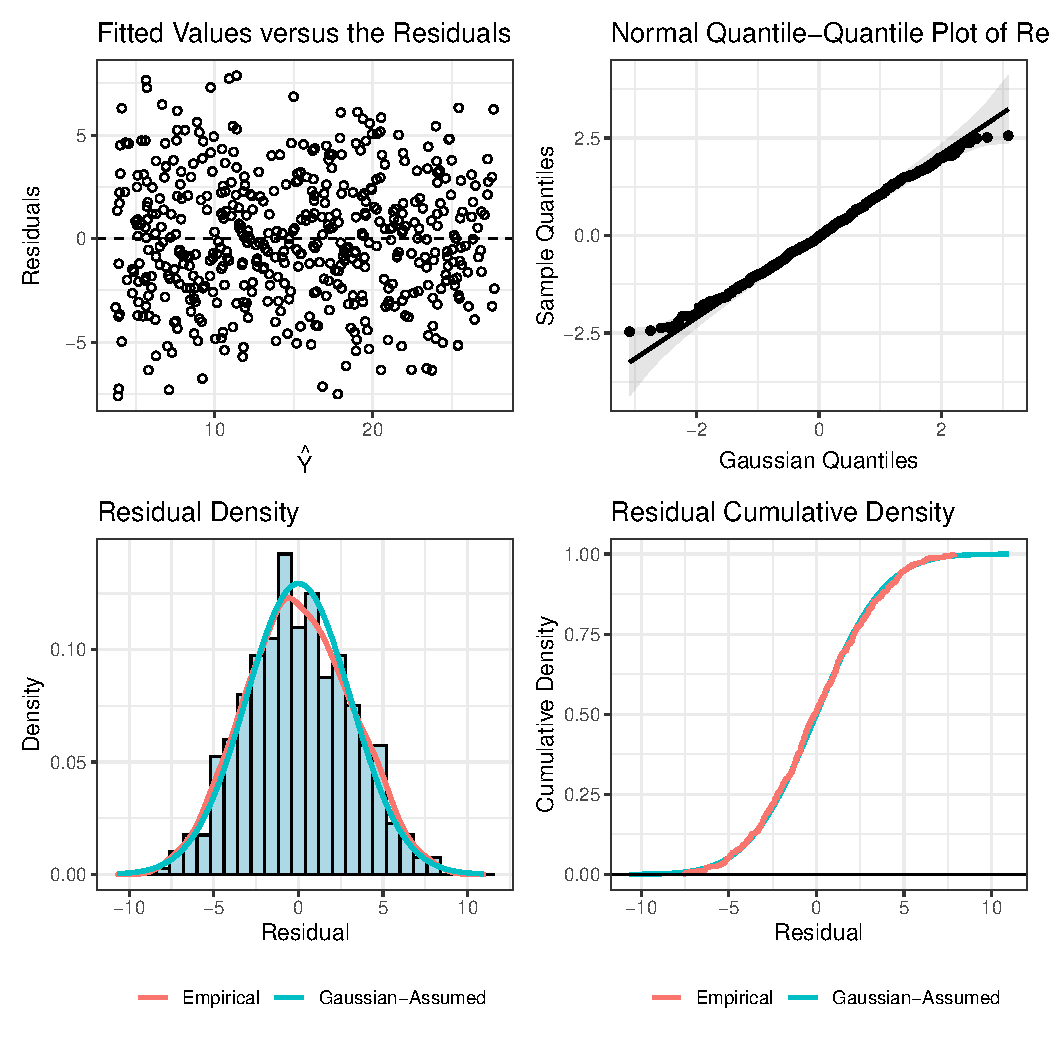
\includegraphics[width=\maxwidth]{figure/unnamed-chunk-15-1} 
\begin{kframe}\begin{alltt}
\hlcom{#Variance is the same}
\hlcom{#https://uc-r.github.io/assumptions_homogeneity#visualization}
\end{alltt}
\end{kframe}
\end{knitrout}
\item Fit a model to the following simulated data, now with added exponential error.
  Make observations about the model equation and the Pearson correlation in relation 
  to the model of part (b).
\begin{knitrout}
\definecolor{shadecolor}{rgb}{0.969, 0.969, 0.969}\color{fgcolor}\begin{kframe}
\begin{alltt}
\hlstd{e}\hlkwb{<-}\hlkwd{rexp}\hlstd{(}\hlkwc{n}\hlstd{=n,}\hlkwc{rate} \hlstd{=} \hlnum{1}\hlopt{/}\hlnum{2}\hlstd{)}
\hlstd{y3}\hlkwb{<-}\hlnum{5}\hlopt{*}\hlstd{x} \hlopt{+} \hlnum{3} \hlopt{+} \hlstd{e}

\hlstd{ggdat}\hlkwb{<-}\hlkwd{data.frame}\hlstd{(}\hlkwc{x}\hlstd{=x,} \hlkwc{y}\hlstd{=y3)}
\hlkwd{ggplot}\hlstd{(ggdat,} \hlkwd{aes}\hlstd{(}\hlkwc{x}\hlstd{=x,} \hlkwc{y}\hlstd{=y))}\hlopt{+}
  \hlkwd{geom_smooth}\hlstd{(}\hlkwc{color}\hlstd{=}\hlstr{"blue"}\hlstd{,}
              \hlkwc{method}\hlstd{=}\hlstr{"lm"}\hlstd{,}
              \hlkwc{formula}\hlstd{=y}\hlopt{~}\hlstd{x)}\hlopt{+}
  \hlkwd{geom_point}\hlstd{(}\hlkwc{shape}\hlstd{=}\hlnum{1}\hlstd{,}
             \hlkwc{alpha}\hlstd{=}\hlnum{.3}\hlstd{)}\hlopt{+}
  \hlkwd{theme_bw}\hlstd{()}
\end{alltt}
\end{kframe}
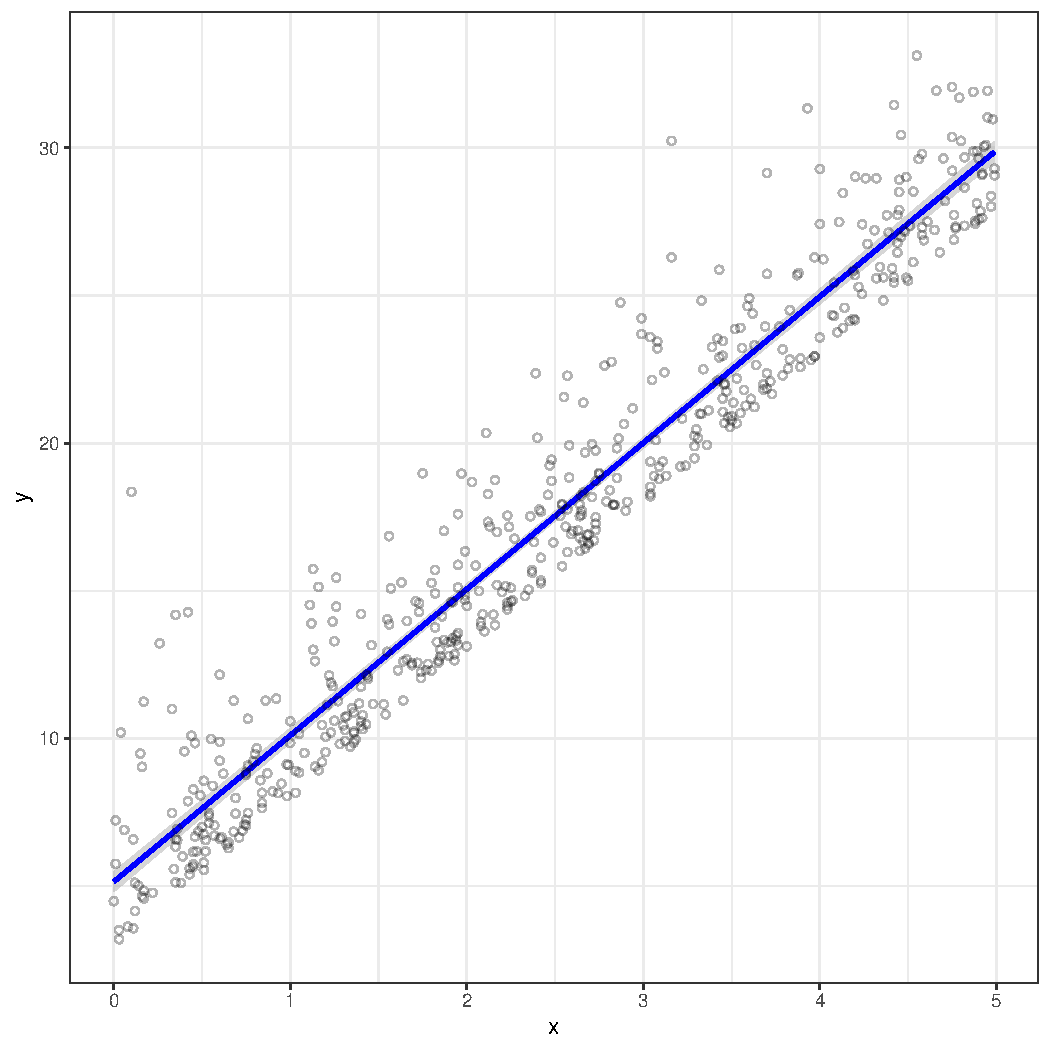
\includegraphics[width=\maxwidth]{figure/unnamed-chunk-16-1} 
\begin{kframe}\begin{alltt}
  \hlcom{#put pearson on the plot}
\hlkwd{cor}\hlstd{(x, y3,} \hlkwc{method}\hlstd{=}\hlstr{"pearson"}\hlstd{)}
\end{alltt}
\begin{verbatim}
## [1] 0.9568558
\end{verbatim}
\end{kframe}
\end{knitrout}

  \item In the model of part (d), evaluate the normality and homogeneity of error 
  terms. Note that we know that common variance is true but we've taken $\epsilon \sim 
  \textrm{exp}(\beta=2)$.
\begin{knitrout}
\definecolor{shadecolor}{rgb}{0.969, 0.969, 0.969}\color{fgcolor}\begin{kframe}
\begin{alltt}
\hlstd{model2} \hlkwb{<-} \hlkwd{lm}\hlstd{(y3}\hlopt{~}\hlstd{x)}
\hlkwd{plotResiduals}\hlstd{(model2)}
\end{alltt}
\end{kframe}
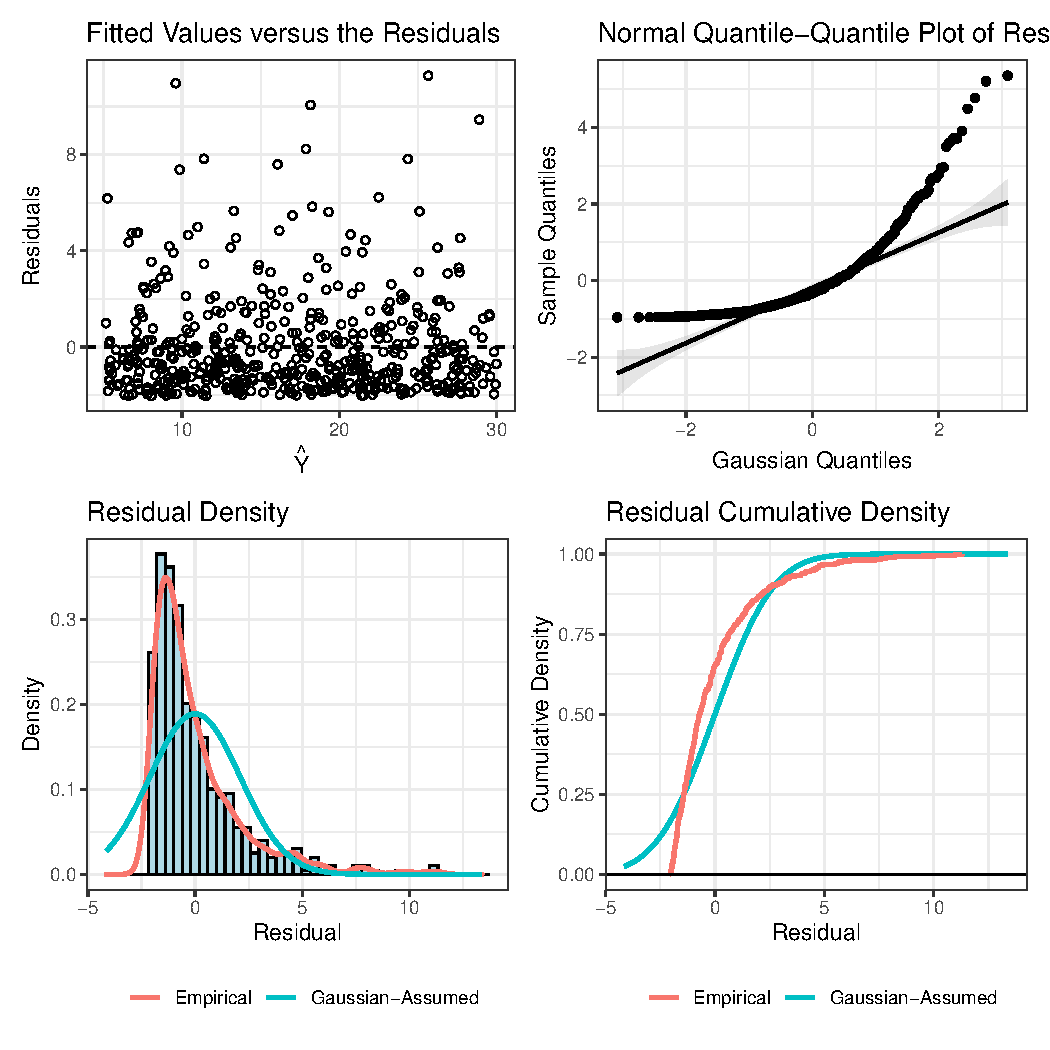
\includegraphics[width=\maxwidth]{figure/unnamed-chunk-17-1} 
\begin{kframe}\begin{alltt}
\hlcom{#It's a skewed normal dist, but it's not homogeneous.}
\end{alltt}
\end{kframe}
\end{knitrout}
\item Fit a model to the following simulated data, now with added Heteroskedastic
normal error. Make observations about the model equation and the Pearson correlation
in relation to the model of part (b).
\begin{knitrout}
\definecolor{shadecolor}{rgb}{0.969, 0.969, 0.969}\color{fgcolor}\begin{kframe}
\begin{alltt}
\hlstd{x4}\hlkwb{<-}\hlstd{x[}\hlkwd{order}\hlstd{(x)]}
\hlstd{e}\hlkwb{<-}\hlkwd{rnorm}\hlstd{(}\hlkwc{n}\hlstd{=n,}\hlkwc{mean}\hlstd{=}\hlnum{0}\hlstd{,}\hlkwc{sd}\hlstd{=}\hlkwd{c}\hlstd{(}\hlkwd{rep}\hlstd{(}\hlnum{1}\hlstd{,n}\hlopt{/}\hlnum{2}\hlstd{),}\hlkwd{rep}\hlstd{(}\hlnum{3}\hlstd{,n}\hlopt{/}\hlnum{2}\hlstd{)))}
\hlstd{y4}\hlkwb{<-}\hlnum{5}\hlopt{*}\hlstd{x4} \hlopt{+} \hlnum{3} \hlopt{+} \hlstd{e}

\hlstd{ggdat}\hlkwb{<-}\hlkwd{data.frame}\hlstd{(}\hlkwc{x}\hlstd{=x4,} \hlkwc{y}\hlstd{=y4)}
\hlkwd{ggplot}\hlstd{(ggdat,} \hlkwd{aes}\hlstd{(}\hlkwc{x}\hlstd{=x,} \hlkwc{y}\hlstd{=y))}\hlopt{+}
  \hlkwd{geom_smooth}\hlstd{(}\hlkwc{color}\hlstd{=}\hlstr{"blue"}\hlstd{,}
              \hlkwc{method}\hlstd{=}\hlstr{"lm"}\hlstd{,}
              \hlkwc{formula}\hlstd{=y}\hlopt{~}\hlstd{x)}\hlopt{+}
  \hlkwd{geom_point}\hlstd{(}\hlkwc{shape}\hlstd{=}\hlnum{1}\hlstd{,}
             \hlkwc{alpha}\hlstd{=}\hlnum{.3}\hlstd{)}\hlopt{+}
  \hlkwd{theme_bw}\hlstd{()}
\end{alltt}
\end{kframe}
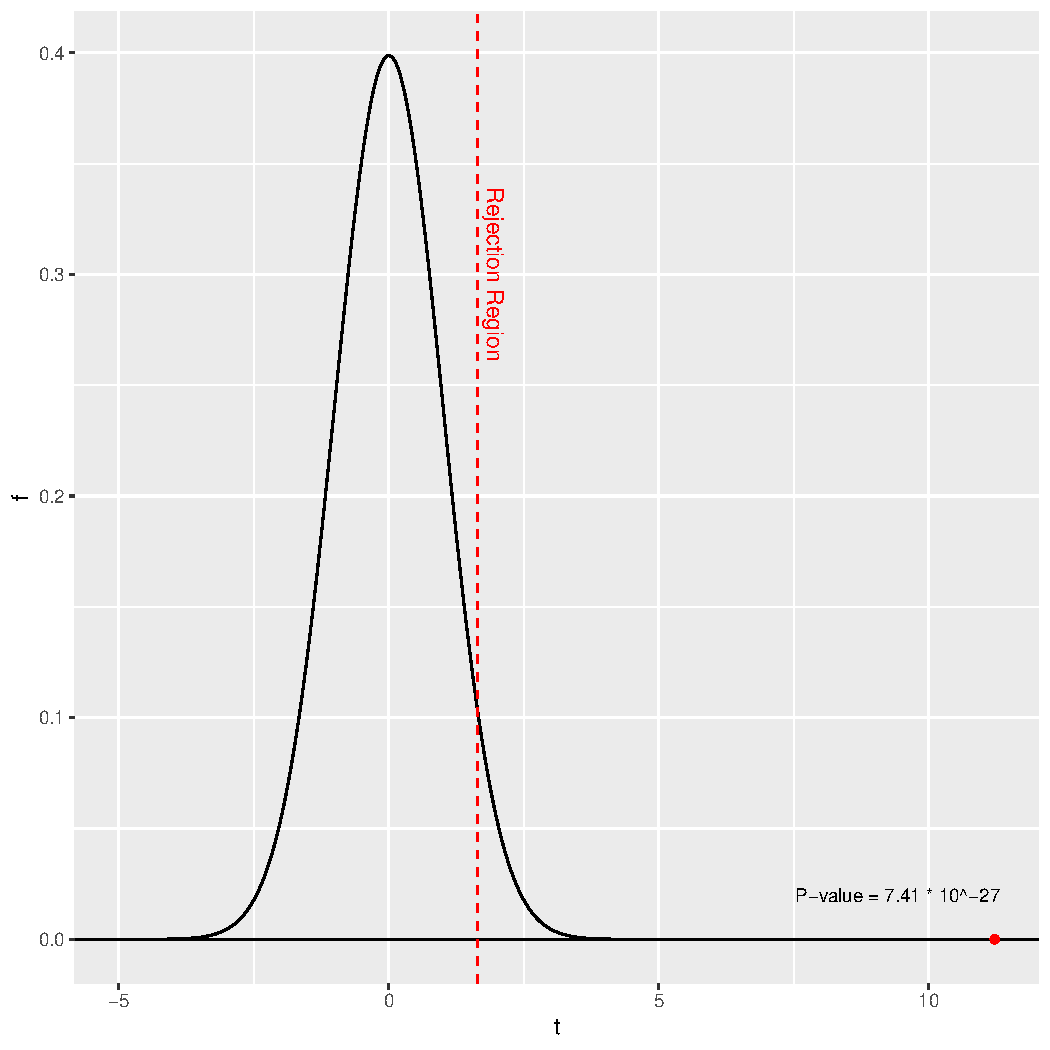
\includegraphics[width=\maxwidth]{figure/unnamed-chunk-18-1} 
\end{knitrout}
  \item In the model of part (f), evaluate the normality and homogeneity of error terms. Note
  that we know that normality of error terms is true, but $\epsilon \sim 
  \textrm{N}(\mu=0,\sigma=1)$ for $x<\widehat{m}$ and $\epsilon \sim 
  \textrm{N}(\mu=0,\sigma=3)$ for $x>\widehat{m}$.
\begin{knitrout}
\definecolor{shadecolor}{rgb}{0.969, 0.969, 0.969}\color{fgcolor}\begin{kframe}
\begin{alltt}
\hlstd{model3} \hlkwb{<-} \hlkwd{lm}\hlstd{(y4}\hlopt{~}\hlstd{x4)}
\hlkwd{plotResiduals}\hlstd{(model3)}
\end{alltt}
\end{kframe}
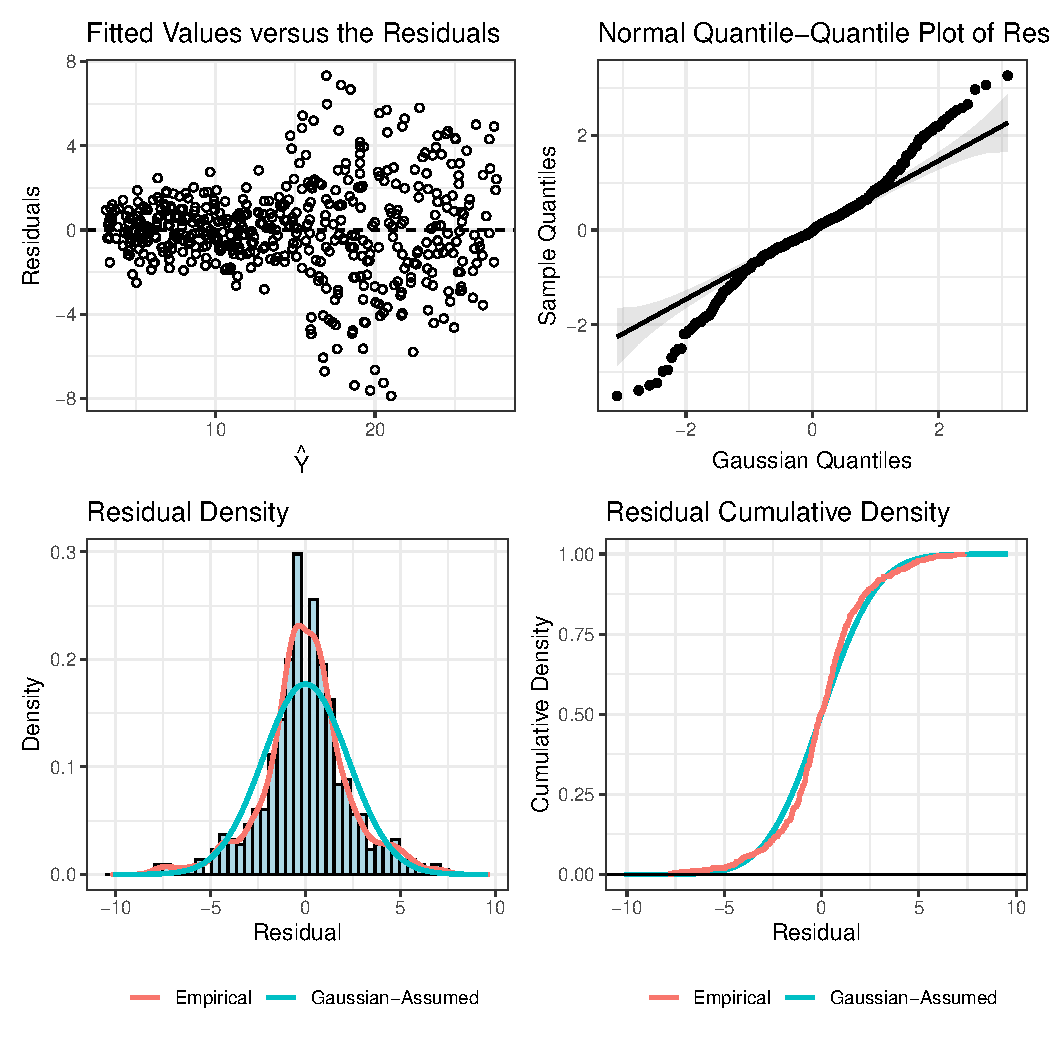
\includegraphics[width=\maxwidth]{figure/unnamed-chunk-19-1} 
\end{knitrout}
\end{enumerate}
%%%%%%%%%%%%%%%%%%%%%%%%%%%%%%%%%%%%%%%%%%%%%%%%%%%%%%%%%%%%%%%%%%%%%%%%%%%%%%%
%%%%%%%%%%%%%%%%%%%%%%%%%%%%%%%%%%%%%%%%%%%%%%%%%%%%%%%%%%%%%%%%%%%%%%%%%%%%%%%
%%%%%%%%%  Question 4
%%%%%%%%%%%%%%%%%%%%%%%%%%%%%%%%%%%%%%%%%%%%%%%%%%%%%%%%%%%%%%%%%%%%%%%%%%%%%%%
%%%%%%%%%%%%%%%%%%%%%%%%%%%%%%%%%%%%%%%%%%%%%%%%%%%%%%%%%%%%%%%%%%%%%%%%%%%%%%%
\item Consider the following simulation.
  \begin{enumerate}
    \item Plot the data simulated below. Assess the linear relationship.
\begin{knitrout}
\definecolor{shadecolor}{rgb}{0.969, 0.969, 0.969}\color{fgcolor}\begin{kframe}
\begin{alltt}
\hlkwd{library}\hlstd{(tidyverse)}
\hlkwd{set.seed}\hlstd{(}\hlnum{7272}\hlstd{)}
\hlstd{n}\hlkwb{<-}\hlnum{50}
\hlstd{ggdat} \hlkwb{<-} \hlkwd{data.frame}\hlstd{(}\hlkwc{x}\hlstd{=}\hlkwd{sample}\hlstd{(}\hlkwc{x}\hlstd{=}\hlkwd{seq}\hlstd{(}\hlnum{0}\hlstd{,}\hlnum{100}\hlstd{,}\hlnum{0.01}\hlstd{),}\hlkwc{size}\hlstd{=n,}\hlkwc{replace}\hlstd{=}\hlnum{TRUE}\hlstd{))} \hlopt
  \hlkwd{mutate}\hlstd{(}\hlkwc{y}\hlstd{=}\hlnum{3.5}\hlopt{+}\hlnum{2.1}\hlopt{*}\hlstd{x}\hlopt{+}\hlkwd{rnorm}\hlstd{(}\hlkwc{n}\hlstd{=n,}\hlkwc{mean}\hlstd{=}\hlnum{0}\hlstd{,}\hlkwc{sd}\hlstd{=}\hlnum{5}\hlstd{))}
\end{alltt}
\end{kframe}
\end{knitrout}
    \item Write out the population model.
\begin{knitrout}
\definecolor{shadecolor}{rgb}{0.969, 0.969, 0.969}\color{fgcolor}\begin{kframe}
\begin{alltt}
\hlcom{#Y=B\{0\}+B\{1\}\{x\} + error}
\end{alltt}
\end{kframe}
\end{knitrout}
    \item Fit the model based on the sample data and write out the sample model below.
\begin{knitrout}
\definecolor{shadecolor}{rgb}{0.969, 0.969, 0.969}\color{fgcolor}\begin{kframe}
\begin{alltt}
\hlcom{#hat(Y)=hat(B\{0\})+hat(B)\{1\}\{x\}}
\hlstd{four.model}\hlkwb{<-}\hlkwd{lm}\hlstd{(y}\hlopt{~}\hlstd{x,} \hlkwc{data}\hlstd{=ggdat)}
\hlkwd{summary}\hlstd{(four.model)}
\end{alltt}
\begin{verbatim}
## 
## Call:
## lm(formula = y ~ x, data = ggdat)
## 
## Residuals:
##      Min       1Q   Median       3Q      Max 
## -11.2855  -2.9153  -0.0545   2.7938  14.7084 
## 
## Coefficients:
##             Estimate Std. Error t value Pr(>|t|)    
## (Intercept)  5.22286    1.44261    3.62 0.000707 ***
## x            2.06056    0.02345   87.89  < 2e-16 ***
## ---
## Signif. codes:  0 '***' 0.001 '**' 0.01 '*' 0.05 '.' 0.1 ' ' 1
## 
## Residual standard error: 5.152 on 48 degrees of freedom
## Multiple R-squared:  0.9938,	Adjusted R-squared:  0.9937 
## F-statistic:  7724 on 1 and 48 DF,  p-value: < 2.2e-16
\end{verbatim}
\begin{alltt}
\hlcom{#hat(B)\{0\}=5.22}
\hlcom{#hat(B)\{1\}\{x\}=2.06}

\hlcom{#hat(Y)=-5.22+2.06x}

\hlcom{#Prediction = 5.22+2.06(x) + (random error)}
\end{alltt}
\end{kframe}
\end{knitrout}
    \item Add the regression line to the plot in black.
\begin{knitrout}
\definecolor{shadecolor}{rgb}{0.969, 0.969, 0.969}\color{fgcolor}\begin{kframe}
\begin{alltt}
\hlkwd{ggplot}\hlstd{(ggdat,} \hlkwd{aes}\hlstd{(}\hlkwc{x}\hlstd{=x,} \hlkwc{y}\hlstd{=y))}\hlopt{+}
  \hlkwd{geom_smooth}\hlstd{(}\hlkwc{color}\hlstd{=}\hlstr{"black"}\hlstd{,}
              \hlkwc{method}\hlstd{=}\hlstr{"lm"}\hlstd{,}
              \hlkwc{formula}\hlstd{=y}\hlopt{~}\hlstd{x)}\hlopt{+}
  \hlkwd{geom_point}\hlstd{(}\hlkwc{shape}\hlstd{=}\hlnum{1}\hlstd{,}
             \hlkwc{alpha}\hlstd{=}\hlnum{.3}\hlstd{)}\hlopt{+}
  \hlkwd{theme_bw}\hlstd{()}
\end{alltt}
\end{kframe}
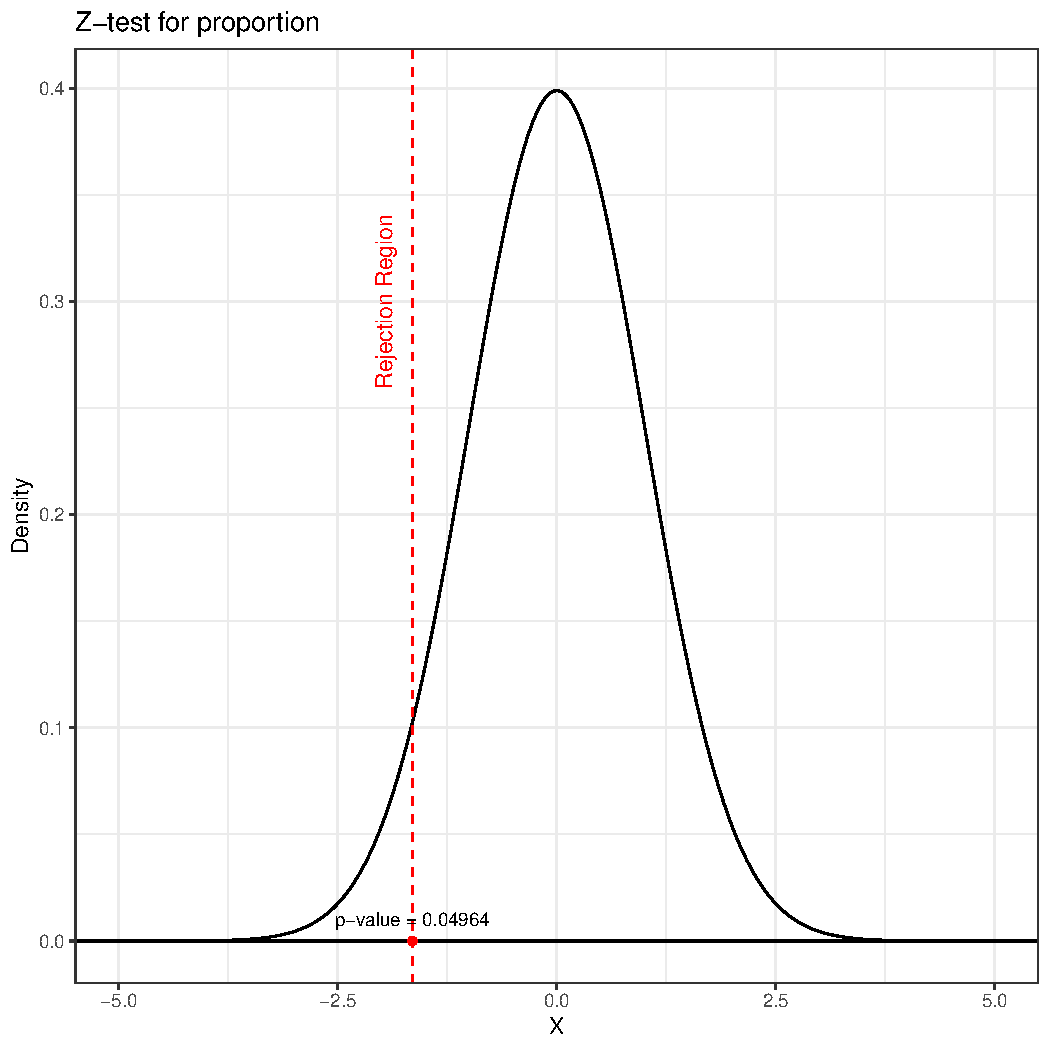
\includegraphics[width=\maxwidth]{figure/unnamed-chunk-23-1} 
\end{knitrout}
    \item Interpret the $R^2$ of the model.
\begin{knitrout}
\definecolor{shadecolor}{rgb}{0.969, 0.969, 0.969}\color{fgcolor}\begin{kframe}
\begin{alltt}
\hlcom{#Adjusted R-squared:  0.9937 }
\hlcom{#99% of the variance can be explained by the model we built.}
\end{alltt}
\end{kframe}
\end{knitrout}
    \item Interpret the overall $F$ test of the model.
\begin{knitrout}
\definecolor{shadecolor}{rgb}{0.969, 0.969, 0.969}\color{fgcolor}\begin{kframe}
\begin{alltt}
\hlcom{#Look at p-value}
\end{alltt}
\end{kframe}
\end{knitrout}
    \item Interpret the coefficients of the model; are they what you would expect?
\begin{knitrout}
\definecolor{shadecolor}{rgb}{0.969, 0.969, 0.969}\color{fgcolor}\begin{kframe}
\begin{alltt}
\hlcom{#Yeah, that's easy.}
\end{alltt}
\end{kframe}
\end{knitrout}
    \item Now, let's add a bad datapoint to the data.
\begin{knitrout}
\definecolor{shadecolor}{rgb}{0.969, 0.969, 0.969}\color{fgcolor}\begin{kframe}
\begin{alltt}
\hlstd{ggdat} \hlkwb{<-} \hlkwd{rbind}\hlstd{(ggdat,}     \hlcom{# original data}
               \hlkwd{c}\hlstd{(}\hlnum{100}\hlstd{,}\hlnum{25}\hlstd{))} \hlcom{# bad observation}
\end{alltt}
\end{kframe}
\end{knitrout}
  \begin{enumerate}
    \item Briefly summarize how adding this data point affects parts (a)-(g).
\begin{knitrout}
\definecolor{shadecolor}{rgb}{0.969, 0.969, 0.969}\color{fgcolor}\begin{kframe}
\begin{alltt}
\hlkwd{ggplot}\hlstd{(ggdat,} \hlkwd{aes}\hlstd{(}\hlkwc{x}\hlstd{=x,} \hlkwc{y}\hlstd{=y))}\hlopt{+}
  \hlkwd{geom_smooth}\hlstd{(}\hlkwc{color}\hlstd{=}\hlstr{"blue"}\hlstd{,}
          \hlkwc{method}\hlstd{=}\hlstr{"lm"}\hlstd{,}
          \hlkwc{formula}\hlstd{=y}\hlopt{~}\hlstd{x)}\hlopt{+}
  \hlkwd{geom_point}\hlstd{(}\hlkwc{shape}\hlstd{=}\hlnum{1}\hlstd{,}
         \hlkwc{alpha}\hlstd{=}\hlnum{.3}\hlstd{)}\hlopt{+}
  \hlkwd{theme_bw}\hlstd{()}
\end{alltt}
\end{kframe}
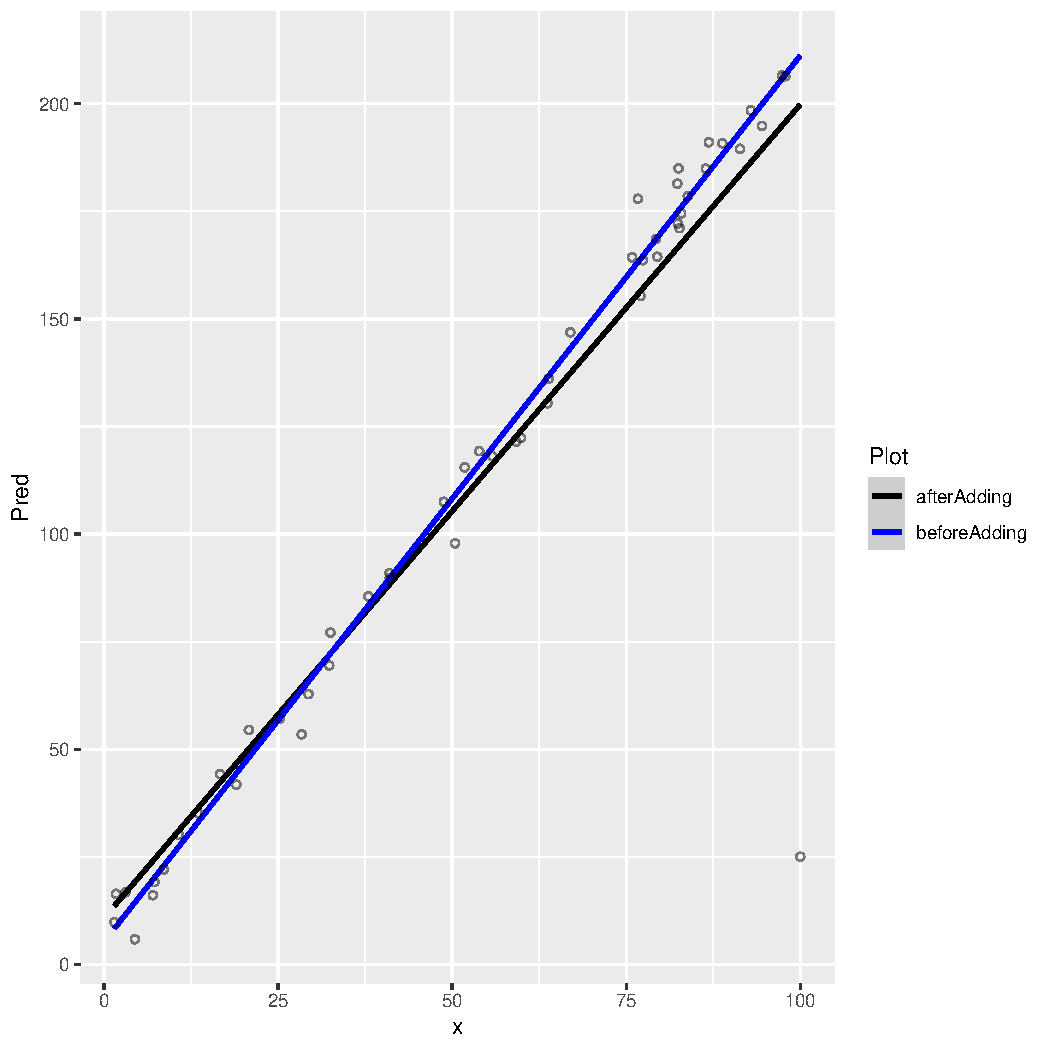
\includegraphics[width=\maxwidth]{figure/unnamed-chunk-28-1} 
\begin{kframe}\begin{alltt}
\hlcom{#there is one unusually small observation!}
\hlstd{four.model}\hlkwb{<-}\hlkwd{lm}\hlstd{(y}\hlopt{~}\hlstd{x,} \hlkwc{data}\hlstd{=ggdat)}
\hlstd{four.model.r} \hlkwb{<-} \hlkwd{rlm}\hlstd{(y}\hlopt{~}\hlstd{x,} \hlkwc{data}\hlstd{=ggdat)}
\end{alltt}


{\ttfamily\noindent\bfseries\color{errorcolor}{\#\# Error in rlm(y \textasciitilde{} x, data = ggdat): could not find function "{}rlm"{}}}\begin{alltt}
\hlkwd{plotResiduals}\hlstd{(four.model)}
\end{alltt}
\end{kframe}
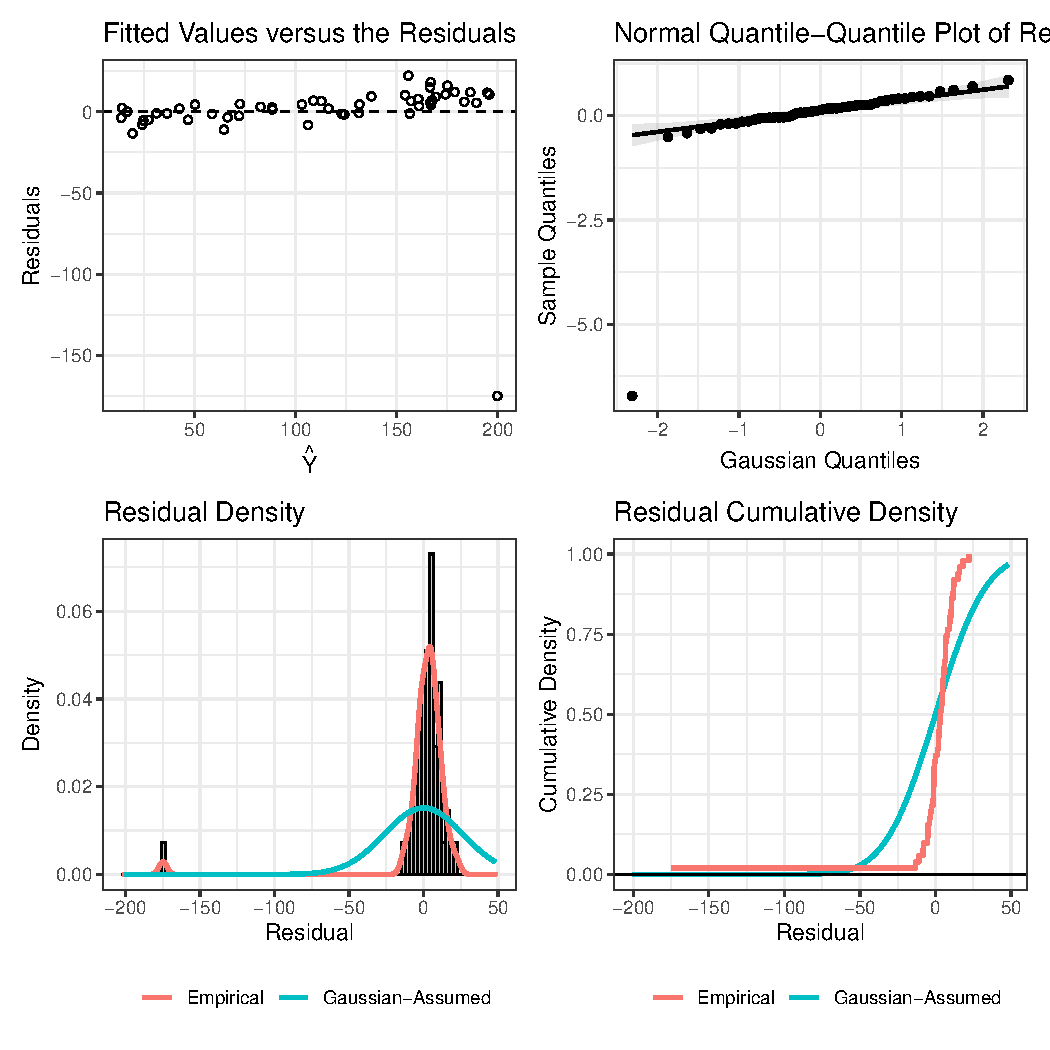
\includegraphics[width=\maxwidth]{figure/unnamed-chunk-28-2} 
\begin{kframe}\begin{alltt}
\hlkwd{summary}\hlstd{(four.model.r)}
\end{alltt}


{\ttfamily\noindent\bfseries\color{errorcolor}{\#\# Error in summary(four.model.r): object 'four.model.r' not found}}\end{kframe}
\end{knitrout}
    \item Add the resulting regression line to the plot in part (d) in blue.
\begin{knitrout}
\definecolor{shadecolor}{rgb}{0.969, 0.969, 0.969}\color{fgcolor}\begin{kframe}
\begin{alltt}
\hlcom{#5.2+(2.06*x)}
\hlcom{#10.742+(1.891*x)}

\hlstd{ggdat.final} \hlkwb{<-} \hlstd{ggdat} \hlopt
  \hlkwd{mutate}\hlstd{(}\hlkwc{beforeAdding} \hlstd{=} \hlnum{5.2}\hlopt{+}\hlstd{(}\hlnum{2.06}\hlopt{*}\hlstd{x),}
     \hlkwc{afterAdding} \hlstd{=} \hlnum{10.742}\hlopt{+}\hlstd{(}\hlnum{1.891}\hlopt{*}\hlstd{x))}\hlopt
  \hlkwd{pivot_longer}\hlstd{(}\hlkwc{cols}\hlstd{=}\hlkwd{ends_with}\hlstd{(}\hlstr{"Adding"}\hlstd{),}
           \hlkwc{names_to}\hlstd{=}\hlstr{"Plot"}\hlstd{,}
           \hlkwc{values_to}\hlstd{=}\hlstr{"Pred"}\hlstd{)}


\hlkwd{ggplot}\hlstd{(ggdat.final,} \hlkwd{aes}\hlstd{(}\hlkwc{x}\hlstd{=x,} \hlkwc{y}\hlstd{=Pred))}\hlopt{+}
  \hlkwd{geom_smooth}\hlstd{(}\hlkwd{aes}\hlstd{(}\hlkwc{color}\hlstd{=Plot),}
          \hlkwc{method}\hlstd{=}\hlstr{"lm"}\hlstd{,}
          \hlkwc{formula}\hlstd{=y}\hlopt{~}\hlstd{x)}\hlopt{+}
  \hlkwd{geom_point}\hlstd{(}\hlkwd{aes}\hlstd{(}\hlkwc{y}\hlstd{=y),} \hlkwc{shape}\hlstd{=}\hlnum{1}\hlstd{,}
         \hlkwc{alpha}\hlstd{=}\hlnum{.3}\hlstd{)}
\end{alltt}
\end{kframe}
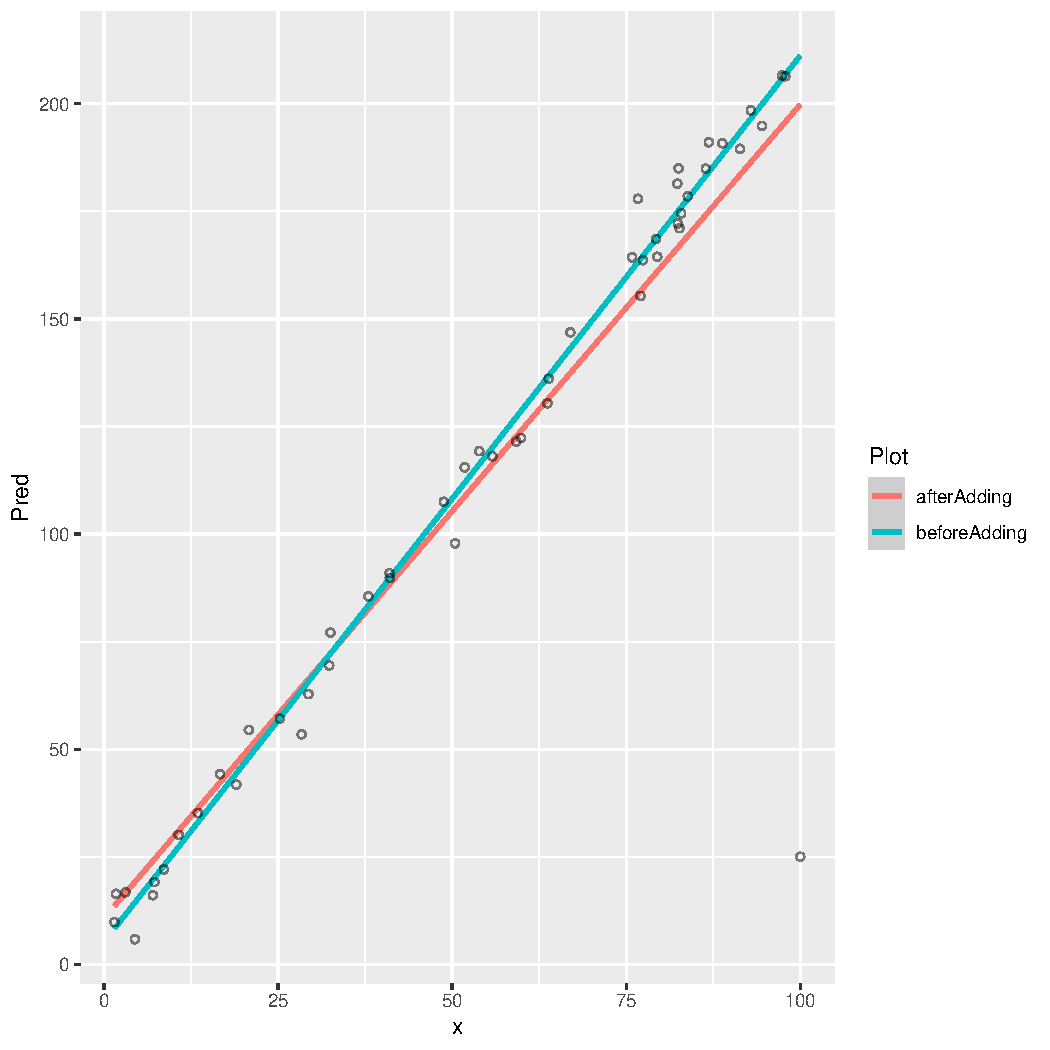
\includegraphics[width=\maxwidth]{figure/unnamed-chunk-29-1} 
\end{knitrout}
    \item Refit this model using several robust techniques for dealing with the
    bad observation. Create a plot that summarizes all the approaches taken, and 
    use a metric to select the best model.

  \end{enumerate}
  \end{enumerate}
%%%%%%%%%%%%%%%%%%%%%%%%%%%%%%%%%%%%%%%%%%%%%%%%%%%%%%%%%%%%%%%%%%%%%%%%%%%%%%%
%%%%%%%%%%%%%%%%%%%%%%%%%%%%%%%%%%%%%%%%%%%%%%%%%%%%%%%%%%%%%%%%%%%%%%%%%%%%%%%
% End File
%%%%%%%%%%%%%%%%%%%%%%%%%%%%%%%%%%%%%%%%%%%%%%%%%%%%%%%%%%%%%%%%%%%%%%%%%%%%%%%
%%%%%%%%%%%%%%%%%%%%%%%%%%%%%%%%%%%%%%%%%%%%%%%%%%%%%%%%%%%%%%%%%%%%%%%%%%%%%%%
\end{enumerate}
\newpage
\bibliography{bib}
\end{document}
